\documentclass[11pt,a4paper]{article}

\usepackage[margin=1in, paperwidth=8.3in, paperheight=11.7in]{geometry}
\usepackage{amsfonts}
\usepackage{amsmath}
\usepackage{amssymb}
\usepackage{enumerate}
\usepackage{enumitem}
\usepackage{fancyhdr}
\usepackage{graphicx}
\usepackage{tikz}
\usepackage{changepage} 

\begin{document}

\pagestyle{fancy}
\setlength\parindent{0pt}
\allowdisplaybreaks

\renewcommand{\headrulewidth}{0pt}

% Cover page title
\title{Combinatorics - Notes}
\author{Dom Hutchinson}
\date{\today}
\maketitle

% Header
\fancyhead[L]{Dom Hutchinson}
\fancyhead[C]{Combinatorics - Notes}
\fancyhead[R]{\today}

% Counters
\newcounter{definition}[section]
\newcounter{example}[section]
\newcounter{notation}[section]
\newcounter{proof}[section]
\newcounter{proposition}[section]
\newcounter{remark}[section]
\newcounter{theorem}[section]

% commands
\newcommand{\dotprod}[0]{\boldsymbol{\cdot}}
\newcommand{\cosech}[0]{\mathrm{cosech}\ }
\newcommand{\cosec}[0]{\mathrm{cosec}\ }
\newcommand{\sech}[0]{\mathrm{sech}\ }
\newcommand{\blocks}[0]{\mathbb{B}}
\newcommand{\nats}[0]{\mathbb{N}}
\newcommand{\real}[0]{\mathbb{R}}
\newcommand{\integers}[0]{\mathbb{Z}}
\newcommand{\nb}[0]{\textit{N.B.} }

\newcommand{\definition}[1]{\stepcounter{definition} \textbf{Definition \arabic{section}.\arabic{definition}\ - }\textit{#1}\\}
\newcommand{\example}[1]{\stepcounter{example} \textbf{Example \arabic{section}.\arabic{example}\ - }\textit{#1}\\}
\newcommand{\notation}[1]{\stepcounter{notation} \textbf{Notation \arabic{section}.\arabic{notation}\ - }\textit{#1}\\}
\newcommand{\proof}[1]{\stepcounter{proof} \textbf{Proof \arabic{section}.\arabic{proof}\ - }\textit{#1}\\}
\newcommand{\proposition}[1]{\stepcounter{proposition} \textbf{Proposition \arabic{section}.\arabic{proposition}\ - }\textit{#1}\\}
\newcommand{\remark}[1]{\stepcounter{remark} \textbf{Remark \arabic{section}.\arabic{remark}\ - }\textit{#1}\\}
\newcommand{\theorem}[1]{\stepcounter{theorem} \textbf{Theorem \arabic{section}.\arabic{theorem}\ - }\textit{#1}\\}

\tableofcontents

% Start of content
\newpage

\section{Counting Techniques}

\proposition{General Approach to Counting Problems}
When presented with a counting problem attempt to split it down into simpler subproblems.\\

\theorem{Bijection Rule}
We can say that a finite, non-empty set $X$ has $n\in\nats$ elements iff there exists a bijection $f:X\to[n]$.\\

\example{Bijection Rule}
How many perfect cubes are there less than $100$?\\
We have that $1^3=1,\ 2^3=8,\ 3^3=27,\ 4^3=64, 5^3=125$.\\
There are 4 perfect cubes less than $100$.\\
A bijection between $X:=\{1,8,27,64\}$ \& $[4]$ is given by $$f:X\to[4]\ st\ f(x)=x^{1/3}$$

\subsection{The Inclusion-Exclusion Principle}

\theorem{Addition Rule}
The number of objects in a set can be counted by splitting the set into disjoint subsets and then adding together the number of objects in each set.\\
\textit{Formally}\\
Let $A_1,\dots,A_n$ be finite pairwise disjoint sets. Then
$$\left|\bigcup\limits_{i=1}^nA_i\right|=\sum_{i=1}^n|A_i|$$

\theorem{Inclusion-Exclusion Theorem}
Let $A_1,\dots,A_n$ be finite sets. Then
$$\left|\bigcup\limits_{i=1}^nA_i\right|=\sum_{i=1}^n|A_i|-\sum_{i_1<i_2}|A_{i_1}\cap A_{i_2}|+\sum_{i_1<i_2<i_3}|A_{i_1}\cap A_{i_2}\cap A_{i_3}|-\dots+(-1)^{n+1}|A_1\cap\dots\cap A_n|$$

\example{Inclusion-Exclusion Theorem}
How many natural numbers are there between 1 and 200 inclusive which are divisible by 3, 5 or 7?\\
Let $D_n$ be the set of natural numbers between 1 and 200 which are divisible by $n$.
\[\begin{array}{lll}
|D_3|=66&|D_5|=40&|D_7|=28\\
|D_{15}|=13&|D_{21}|=9&|D_{35}|=5\\
|D_{105}|=105
\end{array}\]
\[\begin{array}{rcl}
|D_3\cup D_5\cup D_7|&=&(|D_3|+|D_5|+|D_7|)-(|D_{15}|+|D_{21}|+|D_{35}|)+|D_{105}|\\
&=&(66+40+28)-(13+9+5)+1\\
&=&108
\end{array}\]

\subsection{Ordered \& Unordered Selection}

\theorem{Multiplication Rule}
If a counting rule can be split into a number of stages, each of which involves choosing one of a number of options, then the total number of possibilities can be found by multiplying together the number of options at each stage.\\

\example{Multiplication Rule}
Given two non-empty sets $A\ \&\ B$ what is the number of functions with the signature $f:A\to B$?\\
For each element of $A$ there are $|B|$ possible mappings.\\
Hence there are $|B|\times\dots\times|B|$, $|A|$ times, possible functions.\\
This can be simplified to $|B|^{|A|}$.\\

\example{Multiplication Rule}
Given two non-empty finite sets $A\ \&\ B$, what is the number of \textit{injective} functions with the signature $f:A\to B$?\\
For the first element of $A$ we have assigned a value $b\in B$.\\
Then we can map the second element of $A$ to any element in $B\backslash b$, $|B\backslash b|=|B|-1$.\\
This continues for all elements in $A$, meaning the last element of $A$ has $|B|-(|A|-1)$ possible mappings.\\
Provided $|B|\geq|A|$, we have the total number of functions is
$$|B|\times(|B|-1)\times\dots\times(|B|-|A|+1)\equiv(|B|)_{|A|}$$

\subsection{Ordered Statistics}

\definition{Ordered Statistics}
Here we are choosing $k$ objects from a set of $n$ objects.\\
We care about the order that elements are chosen so $\{x_1,x_2\}\not\equiv\{x_2,x_1\}$.\\
There are two cases to this scenario
\begin{itemize}
	\item[-] When repetition is allowed; or,
	\item[-] When repetition is \textbf{not} allowed.
\end{itemize}

\proposition{Repetition is Allowed}
In the case when \textit{Repetition is Allowed} selection is made in $k$ stages.\\
At each stage there are the same $n$ objects to choose from.\\
By the \textit{Multiplication Rule} the total number of choices is
$$n\times\dots\times n=n^k$$

\proposition{Repetition is \textbf{not} Allowed}
In the case when \textit{Repetition is \textbf{not} Allowed} selection is made in $k$ stages.\\
Each stage there is one less option than the stage before.\\
This means that on the $i^{th}$ stage there are $n-(i-1)$ options.\\
By the \textit{Multiplication Rule} the total number of choices is
$$n\times(n-1)\times\dots\times(n-(k-1))=(n)_k$$

\example{Ordered Statistics}
How many five digit octal numbers are there?\\
Since $01234\equiv1234$ there are only 7 options for the first character, but 8 for the rest.\\
Thus there are $7\times8^4$ such numbers.\\
\\
How many such numbers have all distinct digits?\\
The first digit has the same 7 choices. All subsequent digits have a decreasing number of options.\\
Thus there are $7\times7\times6\times5\times4\equiv7\times(7)_4$.

\subsection{Unordered Selection}

\definition{Unordered Selection}
Here we are choosing $k$ objects from a set of $n$ objects.\\
We do \textbf{not} care about the order elements are chosen in. So $\{x_1,x_2\}\equiv\{x_2,x_1\}$.\\
There are two cases to this scenario
\begin{itemize}
	\item[-] When repetition is allowed; or,
	\item[-] When repetition is \textbf{not} allowed.
\end{itemize}

\proposition{Repetition is Allowed}

\proposition{Repetition is \textbf{not} Allowed}
Here we want to find the number of subsets of size $k$.\\

\definition{Binomial Coefficient}
The \textit{Binomial Coefficient} is defined as
$$\begin{pmatrix}n\\k\end{pmatrix}:=\dfrac{(n)_k}{k!}\equiv\dfrac{n!}{(n-k)!k!}$$

\proof{Formula of Binomial Coefficient}
There are $(n)_k$ possible ordered selections of $k$ objects from a set of $n$ objects without repetition.\\
But $k!$ of these represent the same unordered selection.\\

\proposition{Properties of Binomial Coefficient}
The \textit{Binomial Coefficient} has the following properties
\begin{enumerate}[label=\roman*)]
	\item $\begin{pmatrix}n\\k\end{pmatrix}\geq0\ \forall\ n,k\in\nats_0$;
	\item $\begin{pmatrix}n\\k\end{pmatrix}=\begin{pmatrix}n\\n-k\end{pmatrix}$;
	\item $\begin{pmatrix}n\\0\end{pmatrix}=\begin{pmatrix}n\\n\end{pmatrix}=1$; And,
	\item $\begin{pmatrix}n\\k\end{pmatrix}=0$ if $k>n$.
\end{enumerate}

\example{Unordered Selection}
How many ways can we make up a 5-a-side football team, with at most 2 CS students, from 20 maths students \& 15 CS students?\\
$$\begin{pmatrix}15\\2\end{pmatrix}\begin{pmatrix}20\\3\end{pmatrix}+\begin{pmatrix}15\\1\end{pmatrix}\begin{pmatrix}20\\4\end{pmatrix}+\begin{pmatrix}20\\5\end{pmatrix}$$

\proposition{}
Consider the case when \textit{Repetition is Allowed}.\\
For $n\in\nats,\ k\in\nats_0$. The number of
\begin{enumerate}[label=\roman*)]
	\item Unordered selection of $k$ objects from a set of $n$ objects with repetition.
	\item Integer solutions $\{x_1,\dots,x_n\}$ of the equation $x_1+\dots+x_n=k$. st $n_i\geq0\ \forall\ i\in\nats^{\leq k}$.
\end{enumerate}
Is $\begin{pmatrix}n+k-1\\n-1\end{pmatrix}=\begin{pmatrix}n+k-1\\k\end{pmatrix}$, in both cases.\\

\proof{Proposition 1.7}
label the objects in $i)$ with values integer $[1,n]$.\\
let $x_i$ denote the number of times we choose object with label $i$.\\
Then the two problems become the same.\\
Consider placing $k$ blue dots \& $n-1$ red dots in a line, so there are $n+k-1$ possible positions.\\
This corresponds to an n-tuple of non-negative integers where $x_1$ counts the number of blue dots placed before the first red dot, $x_2$ counts the number of blue dots between the first and second red dots etc.\\
This is the same as choosing a set of $n-1$ positions for the red dots from the $x-1+k$ possible position.\\
Thus, there are $\begin{pmatrix}n+k-1\\n-1\end{pmatrix}$ possible choices.\\

\remark{Summary of Ordered \& Unordered Statistics}
The follow table summaries the formulae use for Ordered \& Unordered Statistic problems.\\
\begin{tabular}{c|c|c}
&Ordered&Unordered\\
\hline
With Repetition&$n^k$&$\begin{pmatrix}n+k-1\\n-1\end{pmatrix}$\\
Without Repetition&$(n)_k$&$\begin{pmatrix}n\\k\end{pmatrix}$
\end{tabular}

\subsection{The Binomial Theorem}

\theorem{Pascal's Identity}
$\forall\ i,n\in\nats$ with $i\leq n$ we have that
$$\begin{pmatrix}n\\i\end{pmatrix}=\begin{pmatrix}n-1\\i\end{pmatrix}+\begin{pmatrix}n-1\\i-1\end{pmatrix}$$

\proof{Pascal's Identity}
Fix one element in a set of $n$ elements.\\
Now we can choose set of size $i$ from this set of size $n$ in two mutually exclusive ways
\begin{enumerate}[label=\roman*)]
	\item Choose $i$ elements from the $n-1$ unfixed elements; Or,
	\item Choose the fixed element and $i-1$ elements from the other $n-1$ elements.
\end{enumerate}
In $i)$ there are $\begin{pmatrix}n-1\\i\end{pmatrix}$ choices \& in $ii)$ there are $\begin{pmatrix}n-1\\i-1\end{pmatrix}$ choices.\\
Now apply the addition rule to get $\begin{pmatrix}n\\i\end{pmatrix}=\begin{pmatrix}n-1\\i\end{pmatrix}+\begin{pmatrix}n-1\\i-1\end{pmatrix}$.\\

\theorem{Binomial Theorem}
$\forall\ a,b\ \&\ \forall\ n\in\nats$ we have
$$(a+b)^n=\sum_{j=0}^n\begin{pmatrix}n\\j\end{pmatrix}a^jb^{n-j}$$

\proof{Binomial Theorem}
\textit{This is a proof by induction}.\\
\textit{Base Case}\\
Set $n=1$. Then
$$(a+b)^1=\sum\limits_{j=0}^1\begin{pmatrix}1\\j\end{pmatrix}a^jb^{n-j}=a+b$$
\textit{Inductive Assumption}\\
Assume that for $n\geq1\ (a+b)^n=\sum\limits_{j=0}^n\begin{pmatrix}n\\j\end{pmatrix}a^jb^{n-j}$.\\
\textit{Inductive Case}\\
\[\begin{array}{rcl}
(a+b)^{n+1}&=&(a+b)(a+b)^n\\
&=&(a+b)\sum\limits_{j=0}^n\begin{pmatrix}n\\j\end{pmatrix}a^jb^{n-j}\\
&=&\sum\limits_{j=0}^n\left(\begin{pmatrix}n\\j\end{pmatrix}a^{j+1}b^{n-j}+a^jb^{n-j+1}\right)\\
&=&\begin{pmatrix}n\\0\end{pmatrix}(ab^n+b^{n+1})+\begin{pmatrix}n\\1\end{pmatrix}(a^2b^{n-1}+ab^n)+\dots+\begin{pmatrix}n\\n\end{pmatrix}(a^{n+1}+a^nb)\\
&=&b^{n+1}\begin{pmatrix}n\\0\end{pmatrix}+ab^n\left(\begin{pmatrix}n\\1\end{pmatrix}+\begin{pmatrix}n\\0\end{pmatrix}\right)+\dots+a^nb\left(\begin{pmatrix}n\\n\end{pmatrix}+\begin{pmatrix}n\\n-1\end{pmatrix}\right)+a^{n+1}\begin{pmatrix}n\\n\end{pmatrix}\\
&=&b^{n+1}\begin{pmatrix}n+1\\0\end{pmatrix}+ab^n\begin{pmatrix}n+1\\1\end{pmatrix}+\dots+a^nb\begin{pmatrix}n+1\\n\end{pmatrix}+a^{n+1}\begin{pmatrix}n+1\\n+1\end{pmatrix}\\
&=&\sum\limits_{j=0}^{n+1}\begin{pmatrix}n+1\\j\end{pmatrix}a^jb^{n+1-j}
\end{array}\]
The inductive assumption holds.\\

\theorem{Sum of Binomial Coefficients}
$\forall\ n\in\nats$ we have
$$\sum_{j=0}^n\begin{pmatrix}n\\j\end{pmatrix}=2^n$$

\proof{Sum of Binomial Coefficients}
Set $a=b=1$ in the formula for the Binomial Theorem to get
\[\begin{array}{rcl}
2^n&=&(1+1)^n\\
&=&\sum\limits_{j=0}^n\begin{pmatrix}n\\j\end{pmatrix}1^j1^{n-j}\\
&=&\sum\limits_{j=0}^n\begin{pmatrix}n\\j\end{pmatrix}
\end{array}\]

\proposition{Identity}
$\forall\ j\geq0\ \&\ n\geq1$
$$(j+1)\begin{pmatrix}n\\j+1\end{pmatrix}=n\begin{pmatrix}n-1\\j\end{pmatrix}$$

\proof{Identity}
Consider $h(t)=(1+t)^n$.Then
\[\begin{array}{rcl}
h'(t)&=&n(1+t)^{n+1}\\
&=&n\sum\limits_{j=0}^{n-1}\begin{pmatrix}n-1\\j\end{pmatrix}t^j1^{n-1-j}\\
&=&n\sum\limits_{j=0}^{n-1}\begin{pmatrix}n-1\\j\end{pmatrix}t^j
\end{array}\]
Also by the Binomial Theorem we get
\[\begin{array}{rcl}
h(t)&=&\sum\limits_{j=0}^{n}\begin{pmatrix}n\\j\end{pmatrix}t^j\\
&=&1+\sum\limits_{j=1}^{n}\begin{pmatrix}n\\j\end{pmatrix}t^j
\end{array}\]
Hence
\[\begin{array}{rcl}
h'(t)&=&\sum\limits_{j=1}^n\begin{pmatrix}n\\j\end{pmatrix}jt^{j-1}\\
&=&\sum\limits)_{j=0}^{n-1}\begin{pmatrix}n\\j+1\end{pmatrix}(j+1)t^j
\end{array}\]
By comparing coefficients for both expressions of $h'(t)$ we get
$$(j+1)\begin{pmatrix}n\\j+1\end{pmatrix}=n\begin{pmatrix}n-1\\j\end{pmatrix}$$

\subsection{Pigeon-Hole Principle}

\theorem{Pigeon-Hole Principle}
Let $m>n\geq1$.\\
If there are $m$ pigeons \& $n$ pigeon-holes then at least two pigeons must occupy the same pigeon hole.\\

\theorem{Generalised Pigeon-Hole Principle}
Let $m>nk$ for some $k\in\nats$.\\
If $m$ objects are distributed into $n$ boxes the at least one box must contain at least $k+1$ objects.\\

\example{Generalised Pigeon-Hole Principle}
Show that at least $29$ integers in $[1,200]$ have the same remainder when divided by $7$.\\
Let $S_j=\{i|i\%7=j,\ i\in\nats^{\leq200}\}$.\\
There are $7$ such boxes.\\
It is true that $200>196=28\times7$.\\
By the \textit{Generalised Pigeon-Hole Principle} at least one box must contain $28+1=29$ numbers in it.\\

\section{Generating Functions}

\remark{Motivation}
Here we transform problems about sequences into problems about functions.\\
Thus analyse sequences by manipulating functions.\\

\definition{Generating Function}
Given a sequence of real numbers $(a_n)_{n\geq0}$ we associate it with the formal power series $f(x)=\sum\limits_{n=0}^\infty a_nx^n$.\\
This function is said to be the \textit{Generating Function} of the sequence $(a_n)_{n\geq0}$.
$$(a_0,a_1,a_2,\dots)\rightleftarrows f(x)$$

\example{Polynomial Generating Function}
Consider the sequence $(1,2,3,0,0,\dots)$. Then
$$(1,2,3,0,0,\dots)\rightleftarrows1+2x+3x^2$$

\example{Binomial Theorem Generating Function}
By the \textit{Binomial Theorem} for a fixed $n$ we have
$$(1+x)^n=\sum\limits_{k=0}^n\begin{pmatrix}n\\k\end{pmatrix}x^k=\sum\limits_{k=0}^\infty\begin{pmatrix}n\\k\end{pmatrix}x^k$$
Thus
$$\left(\begin{pmatrix}n\\0\end{pmatrix},\begin{pmatrix}n\\1\end{pmatrix},\dots\right)\rightleftarrows(1+x)^n$$

\proposition{Polynomial Identity}
Consider that $1=(1-x)(1+x+x^2+x^3+\dots)$. Hence
$$\frac{1}{1-x}=1+x+x^2+\dots\implies\frac{1}{1-x}\rightleftarrows(1,1,1,\dots)$$
It follows that $\forall\ m\in\nats$
$$\frac{1}{1-x^m}=1+x^m+x^{2m}+\dots$$
And
$$\frac{1}{1+x}=\frac{1}{1-(-x)}=1-x+x^2-x^3+\dots$$

\subsection{Manipulating Generating Functions}

\theorem{Scaling Rule}
Multiplying a generating function by a constant scalar scales every term in the associated sequence by the same constant.\\
\textit{Formal}\\
\centerline{If $(a_0,a_1,a_2,\dots)\leftrightarrows f(x)\implies(ca_0,ca_1,ca_2,\dots)\leftrightarrows cf(x)$.}\\

\theorem{Addition Rule}
Adding two generating functions together corresponds to adding the corresponding sequences term-by-term.\\
\textit{Formal}\\
\centerline{If $(a_0,a_1,a_2,\dots)\leftrightarrow f(x)$ \& $(b_0,b_1,b_2,\dots)\leftrightarrow g(x)$ then $(a_0+b_0,a_1+b_1,\dots)\leftrightarrow f(x)+g(x)$.}\\

\theorem{Right Shift Rule}
We can add leading zeroes to a sequence by multiplying its generating function by an appropriate power of x.\\
\textit{Formal}\\
\centerline{If $(a_0,a_1,a_2,\dots)\leftrightarrow f(x)$ then $(\underbrace{0,\dots,0}_{k\ times},a_0,a_1,a_2,\dots)\leftrightarrow x^kf(x)$.}

\example{Producing Generating Function}
Find the generating function of $(0,0,0,6,0,6,0,\dots)$.\\
There are $3$ leading 0 so we will multiply the leading generating function by $x^3$.\\
Consider $(1,0,1,0,\dots)$.
$$(1,0,1,0,\dots)\leftrightarrows1+x^2+x^4\equiv\frac{1}{1-x^2}$$
Then
$$(6,0,6,0,\dots)\leftrightarrows\frac{6}{1-x^2}$$
Finally
$$(0,0,0,6,0,6,0,\dots)\leftrightarrows\frac{6x^3}{1-x^2}$$

\theorem{Differentiation Rule}
Differentiating a generating function has the effect that each item of the generated sequence is multiplied by its index \& shifted one place to the left.\\
\textit{Formal}\\
Suppose $(a_0,a_1,a_2,\dots)\leftrightarrows f(x)$.\\
\[\begin{array}{rrcl}
\implies&f(x)&=&\sum\limits_{i=0}^\infty a_ix^i\\
&&=&a_0+\sum\limits_{i=1}^\infty a_ix^i\\
\implies&f'(x)&=&\sum\limits_{i=1}^\infty ia_ix^{i-1}\\
&&=&\sum\limits_{j=1}^\infty(j+1)a_{j+1}x^j
\end{array}\]
Thus $(a_1,2a_2,3a_3,\dots)\leftrightarrows f'(x)$.\\

\example{Differentiation Rule}
Find the generating function of $(n^2)_{n\geq0}$.\\
Note that $(1,1,1,\dots)\leftrightarrows 1+x+x^2+\dots=\frac{1}{1-x}$.\\
By the differentiation rule $(1,2,3,\dots)\leftrightarrows\frac{1}{(1-x)^2}$.\\
By the right-shift rule $(0,1,2,3,\dots)\leftrightarrows\frac{x}{(1-x)^2}$.\\
By the differentiation rule $(1,2^2,3^2,\dots)\leftrightarrows\frac{1}{(1-x)^2}+\frac{2x}{(1-x)^3}=\frac{1+x}{(1-x)^3}$.\\
By the right-shift rule $(0,1^2,2^2,3^2,\dots)\leftrightarrows\frac{x(1+x)}{(1-x)^3}$.\\

\theorem{Convolution Rule}
Taking products of generating functions amounts to taking a convolution of the coefficients.\\
\textit{Formal}\\
Suppose $(a_0,a_1,a_2,\dots)\leftrightarrows f(x)$ \& $(b_0,b_1,b_2,\dots)\leftrightarrows g(x)$.\\
Then $f(x)=\sum_{i=0}^\infty a_ix^i$ \& $g(x)=\sum_{i=0}^\infty b_ix^i$.
$$\implies f(x)g(x)=\left(\sum_{i=0}^\infty a_ix^i\right)\left(\sum_{i=0}^\infty b_ix^i\right)=\sum_{i=0}^\infty c_ix^i$$
where $c_nx^n=a_0b_nx^0x^n+a_1b_{n-1}x^1x^{n-1}+\dots+a_nb_0x^nb^0=\sum_{i=0}^n a_ib_{n-i}x^n$.
Hence $(c_0,c_1,c_2,\dots0\leftrightarrows f(x)g(x)$ where $x_n=\sum){i=0}^n a_ib_{n-i}$.\\

\example{Convolution Rule}
Consider $p(x)=1+x+x^2$ \& $q(x)=1+x+x^2+x^3+x^4$.\\
Note that $p(x)\rightleftarrows(1,1,1,0,\dots)$ \& $q(x)\rightleftarrows(1,1,1,1,1,0,\dots)$.\\
\textit{Find the coefficient of $x^5$ in $p(x)q(x)$}.
\[\begin{array}{rcl}
c_5&=&\sum\limits_{i=0}^5a_ib_{n-i}\\
&=&\left(\sum\limits_{i=0}^0 1\times0\right)+\left(\sum\limits_{i=1}^2 1\times1\right)+\left(\sum\limits_{i=3}^40\times1\right)+\left(\sum\limits_{i=5}^50\times0\right)\\
&=&2\times1=2
\end{array}\]

\subsection{Generating Functions for Counting}

\example{Convolution Rule cont.}
Let $a_i$, the coefficient of $x^i$ in $p(x)$, denote the number of ways I can spend \textsterling$i$. So I can spend 0,1 or 2 pounds.\\
Let $b_i$, the coefficient of $x^i$ in $q(x)$, denote the number of ways Julia can spend \textsterling$i$. So Julia can spend 0,1,2,3 or 5 pounds.\\
In how many ways can be spend \textsterling5 together?\\
This is the coefficient of $x^5$ in $p(x)q(x)$.\\
Which we have shown to be $2$.\\
Furthermore, the combinations are $(1,4)$ \& $(2,3)$.\\

\proposition{General Strategy}
Given a counting problem find a function $f(x)$ such that the coefficient of $x^k$ is its power series expansion in the number of ways of picking $k$ elements in the specified context.\\
\nb The generating function for choosing elements from a series of disjoint sets is the product of the generating functions for each of those sets.\\

\theorem{Power of Sum Identity}
$\forall\ n\in\nats$ we have that
$$\left(\sum_{j=0}^\infty x^j\right)^n=\sum_{k=0}^\infty\begin{pmatrix}n+k-1\\k\end{pmatrix}x^k$$

\proof{Power of Sum Identity}
We have that $\left(\sum_{j=0}^\infty x^j\right)^n=\sum_{k=0}^\infty c_kx^k$ where $\forall\ k\geq0$
\[\begin{array}{rcl}
c_kx^k&=&\sum\limits_{i_1+\dots+i_n=k}x^{i_1}\dots x^{i_n}\\
&=&\sum\limits_{i_1+\dots+i_n=k}x^k\\
&=&x^k\sum\limits_{i_1+\dots+i_n=k}1\\
&=&x^k\begin{pmatrix}n+k-1\\n-1\end{pmatrix}\\
\implies c_k&=&\begin{pmatrix}n+k-1\\n-1\end{pmatrix}=\begin{pmatrix}n+k-1\\k\end{pmatrix}
\end{array}\]

\theorem{Second Identity}
$\forall\ n\in\nats$ we have that
$$\frac{1}{(1-x)^n}=\sum_{k=0}^\infty\begin{pmatrix}n+k-1\\k\end{pmatrix}x^k$$

\example{}
\textit{How many ways are there of choosing 10 ice creams from a selection of 4 flavours?}\\
The sequence for choosing the same type of ice cream is $(1,1,\dots)\leftrightarrows\frac{1}{1-x}$.\\
By the convolution rule, the sequence that counts the number of ways of choosing from 4 different flavours is generated by
$$f(x)=\frac{1}{(1-x)^4}=\sum_{k=0}^\infty\begin{pmatrix}3+k\\k\end{pmatrix}x^k$$
Hence, when $k=10$, the number of choices is $\begin{pmatrix}13\\10\end{pmatrix}$.

\subsection{Generating Functions for Recurrence Relations}

\definition{Recurrence Relation, Sequence}
A sequence $(a_n)_{n\geq0}$ is said to be a \textit{Recurrence Relation} if, for $n$ large enough, $a_n$ is defined as an expression involving previous terms.\\
\nb Generating functions can be used to get an explicit expression for $a_n$ in terms of $n$.\\

\example{Fibonacci Sequence}
The \textit{Fibonacci Sequence} is defined by the recurrence relation
$$a_0=0,\ a_1=1,\ a_n=a_{n-1}+a_{n+2}\ \forall\ n\geq 2$$
\textit{Find an explicit expression for $a_n$}.\\

Let $F(x)$ be the generating function for the \textit{Fibonacci Sequence}. Then
\[\begin{array}{rcl}
F(x)&=&\sum_{n=0}^\infty a_nx^n\\
&=&a_0+a_1x+\sum_{n=2}^\infty (a_{n-1}+a_{n-2})x^n\\
&=&0+x+x\sum_{n=2}^\infty a_{n-1}x^{n-1}+x^2\sum_{n=2}^\infty a_{n-2}x^{n-2}\\
&=&x+x\sum_{m=1}^\infty a_mx^m+x^2\sum_{m=0}^\infty a_mx^m\\
&=&x+x\left(\sum_{m=0}^\infty a_mx^m-0\right)+x^2\sum_{m=0}^\infty a_mx^m\\
&=&x+xF(x)+x^2F(x)\\
(1-x-x^2)F(x)&=&x\\
\implies F(x)&=&\dfrac{x}{1-x-x^2}
\end{array}\]
In finding $a_n$. We see that
\[\begin{array}{rcl}
1-x-x^2&=&-(x^2+x-1)\\
&=&-(x-\frac{1}{2}(-1+\sqrt{5}))(x-\frac{1}{2}(-1-\sqrt{5}))
\end{array}\]
%TODO find & finish

\section{Combinatorial Design}

\definition{Set System}
Let $V$ be a finite set \& $\blocks$ be a collection of subsets of $V$.\\
We call the pair $(V,\blocks)$ a \textit{Set System} with \textit{Ground Set} $V$.\\
\nb Elements of $\blocks$ are referred to as \textit{Blocks}.\\

\definition{K-Uniform}
A \textit{Set System} $(V,\blocks)$ is said to be \textit{k-uniform} if $\forall\ B\in\blocks\ |B|=k$.\\

\example{3-Uniform Set System}
Let $V=\{0,1,2,3,4,5\}$ and\\
$\blocks=\{\{0,1,2\},\{0,2,3\},\{0,3,4\},\{0,4,5\},\{0,1,5\},\{1,2,4\},\{2,3,5\},\{1,3,4\},\{2,4,5\},\{1,3,5\}\}$.\\
Then $(V,\blocks)$ is a \textit{3-uniform} set system with ground set $V$.\\
These blocks can be considered as rotations of the following rotations.\\
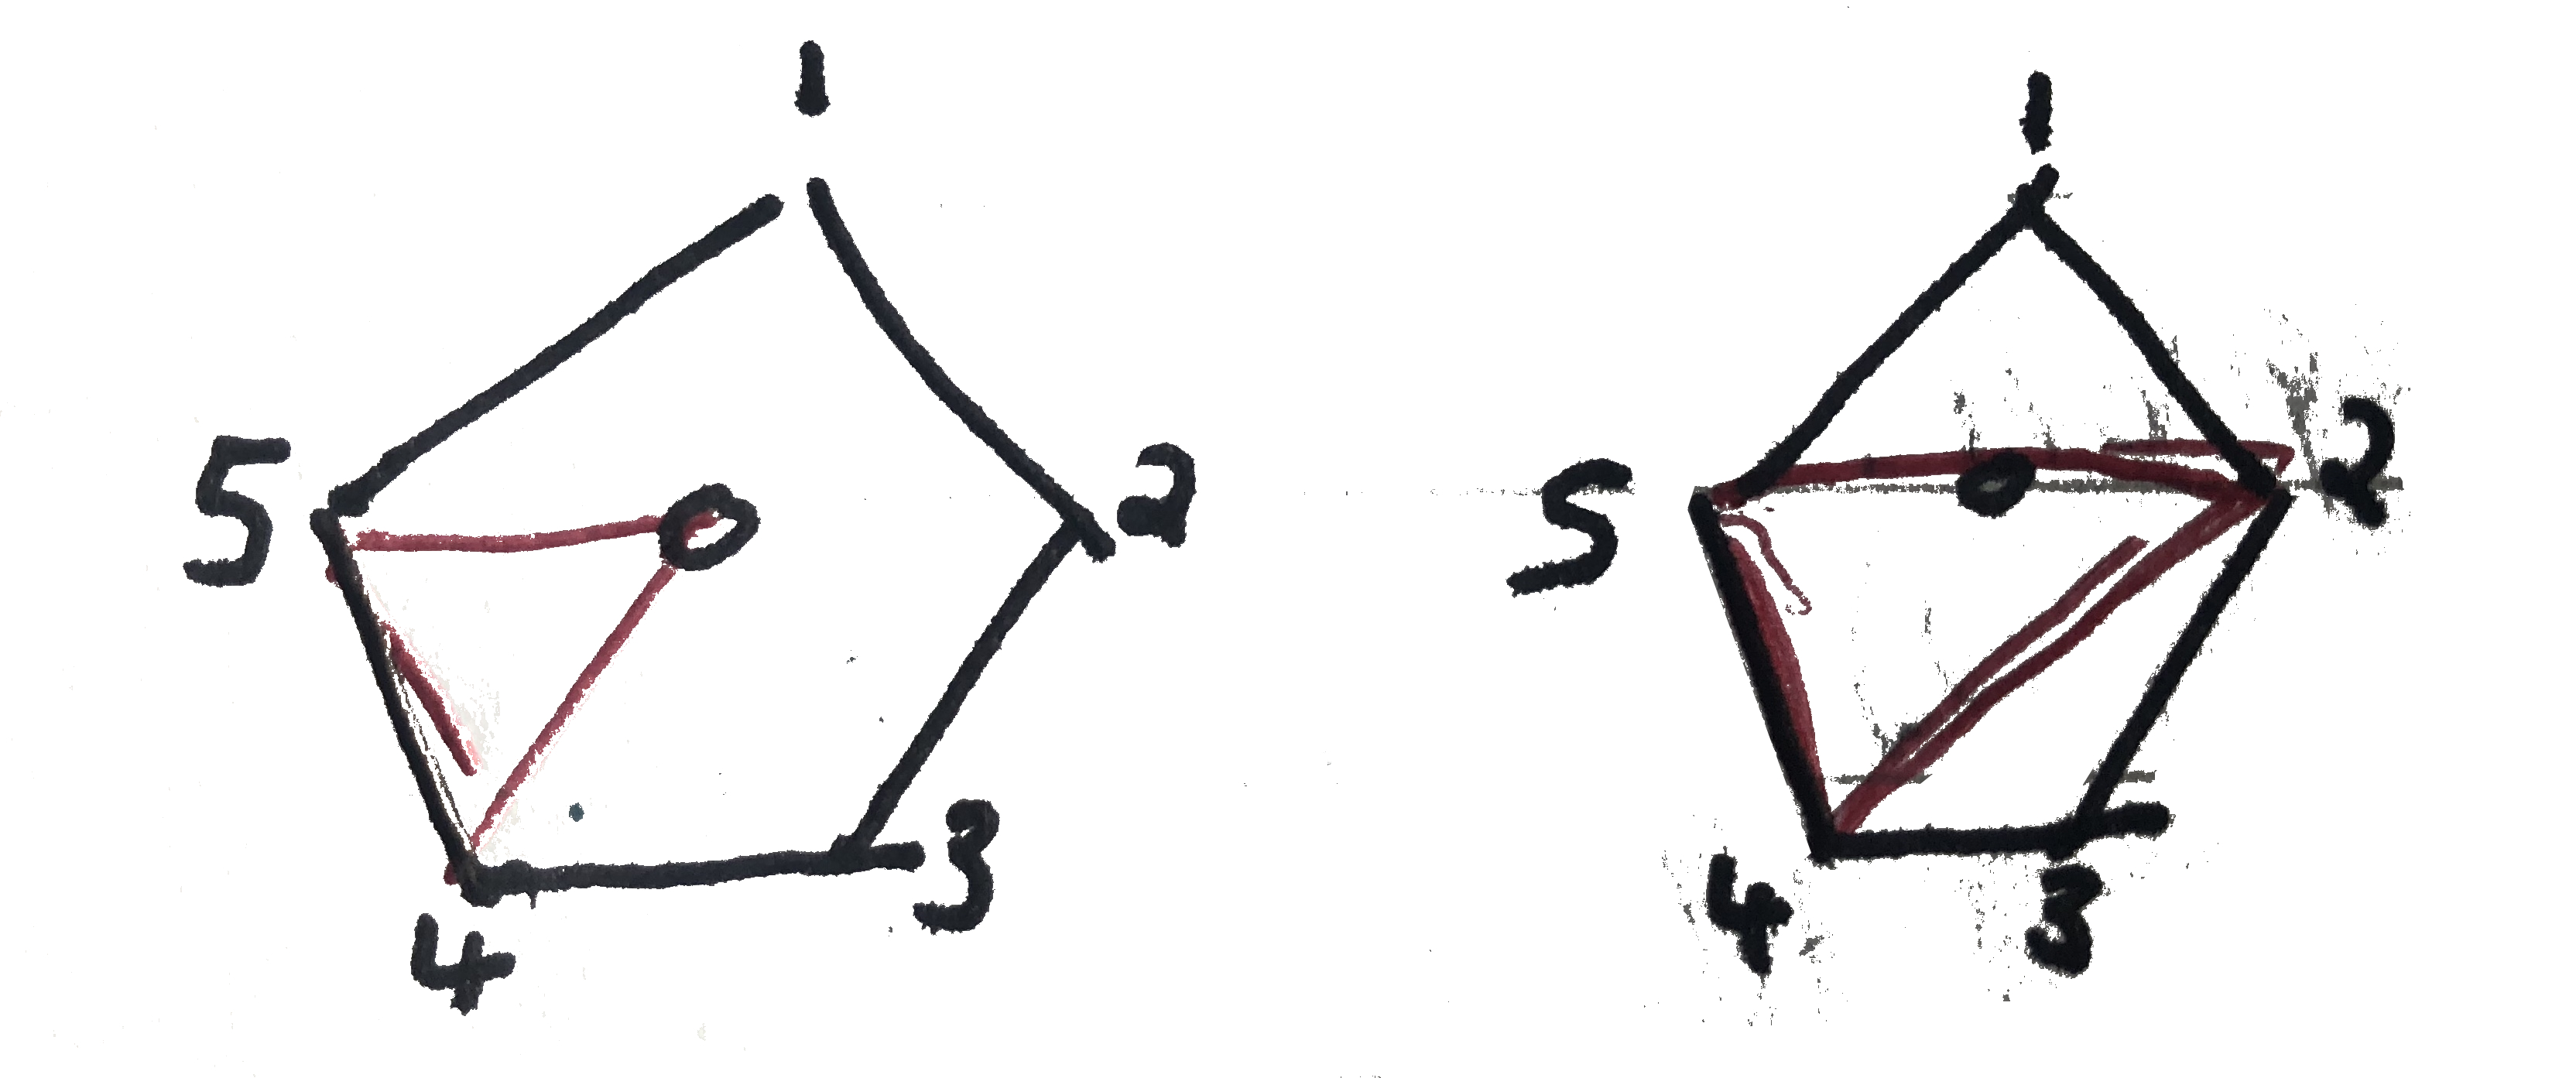
\includegraphics[scale=1]{img/3Uniform.jpg}

\definition{Block Design}
Let $v,k.t,\lambda\in\integers$ with $v\geq k\geq t\geq 1$ \& $\lambda\geq1$.\\
A \textit{Block Design} of type $t-(v,k,\lambda)$ is a set system $(V,\blocks)$ with the following properties
\begin{enumerate}[label=\roman*)]
	\item $|V|=v$;
	\item $\forall\ B\in\blocks\ |B|=k$; (\textit{i.e.} $(V,\blocks)$ is \textit{k-uniform})
	\item Each $T\subset V$ with $|T|=t$ is contained in exactly $\lambda$ elements of $\blocks$.
\end{enumerate}

\example{Disjoint Block Design}
Let $V$ be a set of size $v$ \& let $k\in\nats$ which divides $v$.\\
Partition the elements of $V$ into $\frac{v}{k}$ disjoint subsets of size $k$, namely $B_1,\dots,B_\frac{v}{k}$.\\
Let $\blocks=\{B_1\,\dots,B_\frac{v}{k}\}$.\\
Then $(V,\blocks)$ is a \textit{Block Design} of type $1-(v,l,1)$ since its blocks are disjoint.\\

\example{Block Design}
Let $(V,\blocks)$ be as defined in \textbf{Example 3/1}.\\
Then $(V,\blocks)$ is a $2-(6,3,2)$ block design \& a $1-(6,3,5)$ block design.\\

\definition{Fano Plane}
The \textit{Fano Plane} consists of $V=\{1,2,3,4,5,6,7\}$\\
\& $\blocks=\{\{1,2,3\},\{1,4,7\},\{3,6,7\},\{1,5,6\},\{3,4,5\},\{2,5,7\},\{2,4,6\}\}$.\\
This can be visualised as 7 points in the plane with 7 lines, each passing through exactly 3 points.\\
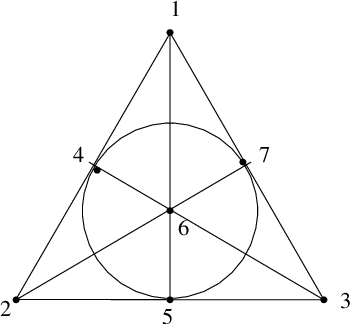
\includegraphics[scale=0.25]{img/fanoplane.png}
\nb The \textit{Fano Plane} is a block design of type $2-(7,3,1)$. It is the smallest example of a \textit{Finite Projection Plane}.\\

\theorem{Number of Blocks in a Block Design}
The number of blocks in a block design of type $t-(v,k,\lambda)$ is
$$b=\frac{\lambda\begin{pmatrix}v\\t\end{pmatrix}}{\begin{pmatrix}k\\t\end{pmatrix}}$$

\proof{Number of Blocks in a Block Design}
\textit{This is a proof by double counting}.\\%Define double counting
Let $N$ be the number of pairs $(T,B)$ where $T$ is a t-element subset of $V$ and $B\in\blocks$ contains $T$.
\begin{enumerate}[label=\roman*)]
	\item By counting $T$ first.\\
	There are $\begin{pmatrix}v\\t\end{pmatrix}$ such subsets $T$.\\
	Each $T$ is contained in $\lambda$ blocks.\\
	So $N=\lambda\begin{pmatrix}v\\t\end{pmatrix}$.
	\item By counting $B$ first.\\
	There are $b$ such blocks.\\
	Each block contains $\begin{pmatrix}k\\t\end{pmatrix}$ sets $T$ of size $t$.\\
	So $N=b\begin{pmatrix}k\\t\end{pmatrix}$.
\end{enumerate}
Thus $\lambda\begin{pmatrix}v\\t\end{pmatrix}=b\begin{pmatrix}k\\t\end{pmatrix}$.
$\implies b=\frac{\lambda\begin{pmatrix}v\\t\end{pmatrix}}{\begin{pmatrix}k\\t\end{pmatrix}}$

\theorem{Replication Number}
In a block design of type $2-(v,k,\lambda)$ every element lies in precisely $r$ blocks where
\begin{enumerate}[label=\roman*)]
	\item $r(k-1)=\lambda(v-1)$; \&
	\item  $bk=vr$.
\end{enumerate}
\nb $r$ stands for \textit{Replication Number}.\\

\proof{Replication Number}
\begin{itemize}
	\item[i)]
	\textit{This is a proof by double counting}.\\
	Fix an arbitrary $v_0\in V$.\\
	Let $N$ be the number of pairs $(T,B)$ with $T$ being a 2-element subset of $V$ which contains $v_0$ \& is a subset of a block.
	\begin{enumerate}
		\item Let's count $T$ first.\\
		There are $v-1$ choices for the element $u\in V$ to make up a 2-element set $T=\{v_0,u\}$.\\
		Each such set $T$ is contained in $\lambda$ blocks of $\blocks$.\\
		Hence $N=\lambda(v-1)$
		\item Now counting $\blocks$ first.\\
		There are $r$ blocks containing $v_0$.\\
		In each such block $B$ there are $k-1$ choices for element $u\in V$ to make up a set $\{v_0,u\}=T\subset B$.\\
		Hence $N=r(k-1)$.
	\end{enumerate}
	Thus $\lambda(v-1)=N=r(k-1)$.
	\item[ii)] Let $M$ be the number of pairs $(u,\blocks)$ with $u\in\blocks$.\\
	Counting $B$ first we have $b$ blocks containing $k$ such elements each.\\
	So $M=bk$.\\
	Counting $u$ first we have $v$ such elements in $V$ and every such $u$ belongs to $r$ blocks.\\
	So $M=vr$.\\
	$\implies bk=vr$.
\end{itemize}

\subsection{Fisher's Inequality}

\definition{Incidence Matrix}
Given a set-system $(V,\blocks)$ with $|V|=v$ \& $|\blocks|=b$ we define its \textit{Incidence Matrix} to be the $v\times b$ matrix $A=(a_{ij})$ whose rows are indexed by the points of $V$ \& its columns are indexed by the points of $\blocks$ and whose entries satisfy
$$a_{ij}=\begin{cases}1&\mathrm{if\ element\ } i \mathrm{\ is\ in\ block\ }j\\0&\mathrm{otherwise}\end{cases}$$

\example{Incidence Matrix of Fano Plane}
Here is the \textit{Incidence Matrix} for the \textit{Fano Plane}
$$A=\begin{pmatrix}1&1&0&1&0&0&0\\1&0&0&0&0&1&1\\1&0&1&0&1&0&0\\0&1&0&0&1&0&1\\0&0&0&1&1&1&0\\0&0&1&1&0&0&1\\0&1&1&0&0&1&0\end{pmatrix}$$
Note that every column contains $k=3$ \textit{'1'}s.\\
Note that every row contains $r=3$ \textit{'1'}s.\\
Note that every pair of rows has $\lambda=1$ \textit{'1'}s in common.\\

\theorem{Fisher's Inequality}
Let $(V,\blocks)$ be a block design of type $2-(v,k,\lambda)$ with $v>k$. Then
$$|\blocks|\geq|V|\equiv b\geq v$$
\nb If $k=1$ then $|\blocks|=|V|$ (\& $\lambda=0$) then trivially we assume below that $k>1$.\\

\proof{Fisher's Inequality}
Let $A-(a_{ij})$ be the incidence matrix of the given block design $(V,\blocks)$ of type $2-(v,k,\lambda)$ with $V=\{x_1,\dots,x_n\}$.\\
\\
Consider the $v\times v$ matrix $M=AA^t$.\\
We want to show that $M$ has rank $v$.\\
Since, trivially, then rank of $A$ \& $A^T$ is at most the number of columns of $A$ (which is $b$).\\
Then if we have $b<v$ we would have
$$v=rank(M)=rank(AA^T)\leq min\{rank(A),rank(A^T)\}\leq b\leq v$$
This is a contradiction.\\
\\We claim that $M$ has rank $v$. Since $M$ has size $x\times v$ it suffices to show that $M$ is non-singular.\\
Or, equivalently, all its columns are linearly independent ($det(M)\neq0$).\\% Define rank
Let $M=(m_{ij})$ then $m_{ij}=$\textit{'$i^{th}$ row of $A$'}$\dotprod$\textit{'$j^{th}$ column of $A^T$'}.\\
Equivalently, $m_{ij}=$\textit{'$i^{th}$ row of $A$'}$\dotprod$\textit{'$j^{th}$ row of $A$'}$=\sum_{k=1}^\infty a_{ik}a_{jk}$.\\
Thus $m_{ij}=$\textit{`Number of sets $B$ that contain both the elements $x_i$ \& $x_j$'}.\\
There are two cases
\begin{enumerate}[label=\roman*)]
	\item $i\neq j$. Then $m_{ij}=\lambda$.
	\item $i=j$. Then $m_{ij}=r+\frac{\lambda(v-1)}{k-1}$.
\end{enumerate}
Hence
$$M=\begin{pmatrix}r&\lambda&\dots&\lambda\\\lambda&r&\dots&\lambda\\\vdots&\vdots&\ddots&\vdots\\\lambda&\lambda&\dots&r\end{pmatrix}$$
Since $det(M)$ is invariant under elementary row operations we apply the follow operations, in succession, $R_1\mapsto R_1+R_2,\dots,R_1\mapsto R_1+R_v$ to get $R_1=\sum_{i=1}^v R_i$. Thus
\[\begin{array}{rcl}
det(M)&=&det\begin{pmatrix}r+(v-1)\lambda&r+(v-1)\lambda&\dots&r+(v-1)\lambda\\\lambda&r&\dots&\lambda\\\vdots&\vdots&\ddots&\vdots\\\lambda&\lambda&\dots&r\end{pmatrix}\\
&=&[r+(v-1)\lambda]det\begin{pmatrix}1&1&\dots&1\\\lambda&r&\dots&\lambda\\\vdots&\vdots&\ddots&\vdots\\\lambda&\lambda&\dots&r\end{pmatrix}\\
&=&[r+(v-1)\lambda]det\begin{pmatrix}1&1&1&\dots&1\\
0&(r-\lambda)&0&\dots&0\\\vdots&\vdots&\vdots&\ddots&\vdots\\0&0&0&\dots&(r-\lambda)\end{pmatrix}\\
&=&[r+(v-1)\lambda](r-\lambda)^{v-1}
\end{array}\]
The final statement uses $R_i\mapsto R_i-\lambda R_1$ for each $i=2,\dots,v$.\\
\\
But $v>k$ so $\frac{v-1}{k-1}>1$.\\
Thus $r-\lambda>0$.\\
Also $r>0$ \& $(v-1)\lambda\geq0$.\\
So $r+(v-1)\lambda>0$.\\
Thus $det(M)=[r+(v-1)\lambda](r-\lambda)^{v-1}>0$\\
This proves $M$ is not singular \& thus our claim holds and the theorem is proved.\\

\example{Fisher's Inequality}
By \textit{Fisher's Inequality} there is no block design of type $2-(25,10,3)$.\\
Indeed, by \textbf{Theorem 3.1}, the number of blocks would be
$$b=\frac{\lambda\begin{pmatrix}v\\t\end{pmatrix}}{\begin{pmatrix}k\\t\end{pmatrix}}=\frac{3\begin{pmatrix}25\\10\end{pmatrix}}{\begin{pmatrix}10\\2\end{pmatrix}}=\frac{3\times25\times24}{10\times9}=20$$
but $b=20<25=v$ which violates \textit{Fisher's Inequality}.\\

\section{Introduction to Graph Theory}

\definition{Graph}
A \textit{Graph}, $G$, is an ordered pair $(V,R)$ where $V$ is a set \& $E$ is a set of two-element subsets of $V$.\\
The elements of $V$ are called \textit{Vertices} of $G$.\\
The elements of $E$ are called \textit{Edges} of $G$.\\
\nb Vertices are sometimes called nodes.\

\definition{Order of a Graph}
The \textit{Order} of a graph $(V,E)$ is the the size of $V$ (number of vertices).\\

\definition{Simple Graph}
A \textit{Simple Graph} is an unweighed, undirected graph which contains no edges which start \& end on the same node, nor multiple edges between the same pair of vertices.\\

\remark{Graphs as Set Systems}
Graphs are \textit{2-uniform set systems}.\\

\definition{Adjacency}
Let $G=(V,E)$ be a graph. Suppose $u,v\in V$ \& $\{u,v\}\in E$.\\
We say that $u$ \& $v$ are adjacent in $G$, or $u$ is a neighbour to $v$ (\& visa versa).\\
\nb Adjacency is not reflexive or transitive, so is not an equivalence relation.\\

\definition{Neighbourhood \& Degree}
Let $G=(V,E)$ be a graph. Let $v\in V$.\\
The \textit{Neighbourhood of $v$}, $N_G(v)$, is the set of neighbours of $v$ in $G$.\\
The \textit{Degree of $v$}, $deg_G(v)$,  is the number of neighbours of $v$ in $G$.\\
\nb $deg_G(v)=|N_G(v)|$.\\

\subsection{Common Graphs}

\definition{Complete Graph}
A \textit{Complete Graph} of order $n$, $K_n$, has vertex set $\{x_1,\dots,x_n\}$ \& edge set $\{\{x_i,x_j\}|i\neq j,\ i,j\in[1,n]\}$.\\
A complete graph of $n$ edges always has the maximum number of possible edges $\begin{pmatrix}n\\2\end{pmatrix}$.\\

\example{Complete Graph, $K_4$}
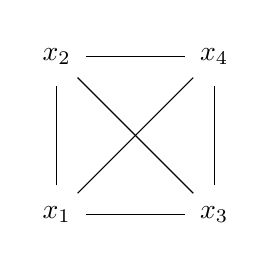
\begin{tikzpicture}
	\node[shape=circle] (1) at (0,0) {$x_1$};
	\node[shape=circle] (2) at (0,2) {$x_2$};
	\node[shape=circle] (3) at (2,0) {$x_3$};
	\node[shape=circle] (4) at (2,2) {$x_4$};
	
	\path [-] (1) edge (2);
	\path [-] (1) edge (3);
	\path [-] (1) edge (4);
	\path [-] (2) edge (3);
	\path [-] (2) edge (4);
	\path [-] (3) edge (4);
\end{tikzpicture}

\definition{Path}
A \textit{Path} of length $n$, $P_n$ is defined to have vertex set $V=\{x_1,\dots,x_{n+1}\}$ \& edge set $\{\{x_i,x_{i+1}|i\in[1,n]\}$.\\
\nb \textit{Path}s have no repeated edges.\\

\example{Path, $P_4$}
\begin{tikzpicture}
	\node[shape=circle] (1) at (0,0) {$x_1$};
	\node[shape=circle] (2) at (1,2) {$x_2$};
	\node[shape=circle] (3) at (2,0) {$x_3$};
	\node[shape=circle] (4) at (3,2) {$x_4$};
	\node[shape=circle] (5) at (4,0) {$x_5$};
	
	\path [-] (1) edge (2);
	\path [-] (2) edge (3);
	\path [-] (3) edge (4);
	\path [-] (4) edge (5);
\end{tikzpicture}

\definition{Cycle}
A \textit{Cycle} of length $n$, $C_n$, is obtained by adding the edge $\{x_1,x_n\}$ to a simple path of length $n-1$.\\

\example{Cycle, $C_5$}
\begin{tikzpicture}
	\node[shape=circle] (1) at (0,0) {$x_1$};
	\node[shape=circle] (2) at (1,2) {$x_2$};
	\node[shape=circle] (3) at (2,1) {$x_3$};
	\node[shape=circle] (4) at (3,2) {$x_4$};
	\node[shape=circle] (5) at (4,0) {$x_5$};
	
	\path [-] (1) edge (2);
	\path [-] (2) edge (3);
	\path [-] (3) edge (4);
	\path [-] (4) edge (5);
	\path [-] (5) edge (1);	
\end{tikzpicture}

\definition{Tree}
A \textit{Tree} is a graph with no cycles.\\

\example{Tree}
\begin{tikzpicture}
	\node[shape=circle] (1) at (0,0) {$x_1$};
	\node[shape=circle] (2) at (-1,-1) {$x_2$};
	\node[shape=circle] (3) at (0,-1) {$x_3$};
	\node[shape=circle] (4) at (1,-1) {$x_4$};
	\node[shape=circle] (5) at (0,-2) {$x_5$};
	\node[shape=circle] (6) at (2,-2) {$x_6$};
	
	\path [-] (1) edge (2);
	\path [-] (1) edge (3);
	\path [-] (1) edge (4);
	\path [-] (4) edge (5);
	\path [-] (4) edge (6);	
\end{tikzpicture}

\definition{Star}
A \textit{Star} on $n$ vertices has vertex set $V=\{x_1,\dots,x_n\}$ \& edge set $E=\{\{x_1,x_i\}:i\in[2,n]\}$.\\

\example{Star, 7}
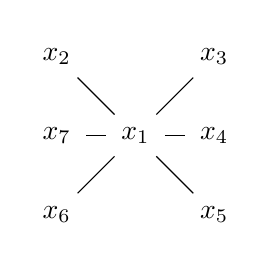
\begin{tikzpicture}
	\node[shape=circle] (1) at (0,0) {$x_1$};
	\node[shape=circle] (2) at (-1,1) {$x_2$};
	\node[shape=circle] (3) at (1,1) {$x_3$};
	\node[shape=circle] (4) at (1,0) {$x_4$};
	\node[shape=circle] (5) at (1,-1) {$x_5$};
	\node[shape=circle] (6) at (-1,-1) {$x_6$};
	\node[shape=circle] (7) at (-1,0) {$x_7$};
	
	\path [-] (1) edge (2);
	\path [-] (1) edge (3);
	\path [-] (1) edge (4);
	\path [-] (1) edge (5);
	\path [-] (1) edge (6);	
	\path [-] (1) edge (7);	
\end{tikzpicture}

\subsection{Basic Properties of Graphs}

\definition{Graph Isomorphism}
Let $G_1=(V_1,E_1)$ \& $G_2=(V_2,E_2+$ be graphs.\\
$G_1$ \& $G_2$ are isomorphic if $\exists$ a bijection $\phi:V_1\to V_2$ st
$$\ \forall\ u,v\in V_1,\ \{u,v\}\in E_1, \{\phi(u),\phi(v)\}\in E_2$$

\example{Isomorphic Graphs}
The following two graphs are isomorphic\\
\begin{tikzpicture}
	\node[shape=circle] (1) at (0,0) {$1$};
	\node[shape=circle] (2) at (2,-1) {$2$};
	\node[shape=circle] (3) at (1,-3) {$3$};
	\node[shape=circle] (4) at (-1,-3) {$4$};
	\node[shape=circle] (5) at (-2,-1) {$5$};
	
	\path [-] (1) edge (2);
	\path [-] (2) edge (3);
	\path [-] (3) edge (4);
	\path [-] (4) edge (5);
	\path [-] (5) edge (1);
\end{tikzpicture}
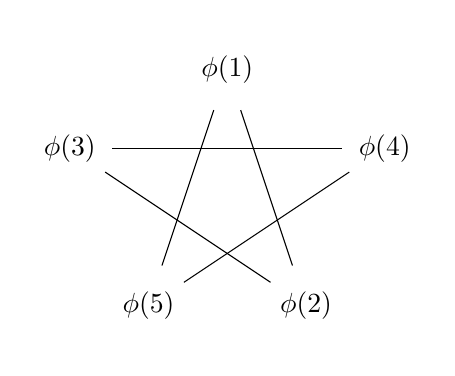
\begin{tikzpicture}
	\node[shape=circle] (1) at (0,0) {$\phi(1)$};
	\node[shape=circle] (2) at (2,-1) {$\phi(4)$};
	\node[shape=circle] (3) at (1,-3) {$\phi(2)$};
	\node[shape=circle] (4) at (-1,-3) {$\phi(5)$};
	\node[shape=circle] (5) at (-2,-1) {$\phi(3)$};
	
	\path [-] (1) edge (3);
	\path [-] (3) edge (5);
	\path [-] (5) edge (2);
	\path [-] (2) edge (4);
	\path [-] (4) edge (1);
\end{tikzpicture}\\

\definition{Degree Sequence}
Let $G=(V,E)$ be a graph on n vertices.\\
Label the vertices $x_1,\dots,x_n$ in order of non-decreasing degree.\\
The \textit{Degree Sequence} of $G$ is the sequence $(deg_G(x_1),\dots,deg_G(x_n))$.\\

\proposition{Invariants}
Establishing whether two graphs are isomorphic is hard.\\
We use invariants to make this easier
\begin{enumerate}[label=\roman*)]
	\item Two isomorphic graphs have the same number of edges;
	\item Two isomorphic graphs have the same degree sequence.
\end{enumerate}

\example{Degree Sequence}
In the previous example both graphs have \textit{Degree Sequence}
$$(2,2,2,2,2)$$

\theorem{Handshaking Lemma}
The sum of the degrees of the vertices in a graph is equal to twice the number of edges.
$$\sum_{v\in V}deg_G(v)=2|E|$$

\proof{Handshaking Lemma}
Let $N$ be the number of pairs $(v,e)$ where $v\in V,\ e\in E\ \&\ v\in e$.
\begin{enumerate}[label=\roman*)]
	\item Counting vertices first we get $N=\sum_{v\in V}deg_G(v)$.
	\item Counting edges first we see each edge has two vertices so $N=2|E|$.
\end{enumerate}
Thus $\sum_{v\in V}deg_G(v)=N=2|E|$.\\

\definition{Sub-graph}
A \textit{Sub-graph} $G'=(V',E')$ of a graph $G=(V,E)$ is a graph whose
$$V'\subseteq V\ \&\ E'\subseteq \{\{u,v\}:\{u,v\}\in E;\ u,v\in V'\}$$

\example{Sub-graph}
The cycle $C_4$ is a subgraph of the graph below.\\
\begin{tikzpicture}
	\node[shape=circle] (1) at (0,0) {1};
	\node[shape=circle] (2) at (2,0) {2};
	\node[shape=circle] (3) at (4,0) {3};
	\node[shape=circle] (4) at (-0,-2) {4};
	\node[shape=circle] (5) at (2,-2) {5};
	
	\path [-] (1) edge (2);
	\path [-] (2) edge (3);
	\path [-] (2) edge (5);
	\path [-] (5) edge (4);
	\path [-] (4) edge (1);
	\path [-] (4) edge (2);
\end{tikzpicture}
\begin{tikzpicture}
	\node[shape=circle] (1) at (0,0) {1};
	\node[shape=circle] (2) at (2,0) {2};
	\node[shape=circle] (4) at (-0,-2) {4};
	\node[shape=circle] (5) at (2,-2) {5};
	
	\path [-] (1) edge (2);
	\path [-] (2) edge (5);
	\path [-] (5) edge (4);
	\path [-] (4) edge (1);
\end{tikzpicture}

\definition{Induced Sub-graph}
We say $G'$ is an \textit{Induced Sub-graph} of $G$ if
\begin{enumerate}[label=\roman*)]
	\item $V'\subseteq V$; and,
	\item $E'=\{\{u,v\}:\{u,v\}\in E;\ u,v\in V'\}$.
\end{enumerate}

\example{Sub-graph}
The right-hand graph is a sub-graph of the left-hand graph.\\
\begin{tikzpicture}
	\node[shape=circle] (1) at (0,0) {1};
	\node[shape=circle] (2) at (2,0) {2};
	\node[shape=circle] (3) at (4,0) {3};
	\node[shape=circle] (4) at (-0,-2) {4};
	\node[shape=circle] (5) at (2,-2) {5};
	
	\path [-] (1) edge (2);
	\path [-] (2) edge (3);
	\path [-] (2) edge (5);
	\path [-] (5) edge (4);
	\path [-] (4) edge (1);
	\path [-] (4) edge (2);
\end{tikzpicture}
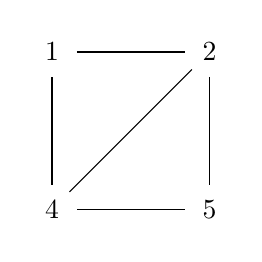
\begin{tikzpicture}
	\node[shape=circle] (1) at (0,0) {1};
	\node[shape=circle] (2) at (2,0) {2};
	\node[shape=circle] (4) at (-0,-2) {4};
	\node[shape=circle] (5) at (2,-2) {5};
	
	\path [-] (1) edge (2);
	\path [-] (2) edge (5);
	\path [-] (5) edge (4);
	\path [-] (4) edge (1);
	\path [-] (4) edge (2);
\end{tikzpicture}

\definition{Path as a Sub-graph}
A sub-graph of a graph $G$ which is isomorphic to a path $P_t$ for $t\geq 0$ is called a \textit{Path in G}.\\
\nb This allows for the trivial path of a node to itself in 0 steps.\\
\nb All vertices are distinct.\\

\definition{Cycle}
A sub-graph of a graph $G$ which is isomorphic to a cycle $C_t$ for $t\geq 3$ is called a \textit{Cycle in G}.\\
\nb All vertices are distinct.\\

\definition{Connected Vertices}
A pair of vertices in a graph are said to be \textit{Connected} when $\exists$ a path that begins at one \& ends at the other.\\
\nb By convention a vertex is said to be connected to itself by the path $P_0$.\\

\remark{Equivalence Relation Between Vertices}
For a graph $G=(V,E)$ \& $x,y\in V$ there is an equivalent relation $x\simeq y$ if they are connected.\\

\definition{Connected Graph}
A graph is said to be \textit{Connected} when every pair of vertices in its vertex set are \textit{Connected}.\\

\definition{Connected Component}
A \textit{Connected Component} of a graph is a maximally connected sub-graph of $G$.\\
\nb Connected components of a graph are equivalence classes.\\

\example{Connection}
Consider the following graph\\
\begin{tikzpicture}
	\node[shape=circle] (1) at (0,0) {1};
	\node[shape=circle] (2) at (2,0) {2};
	\node[shape=circle] (3) at (4,0) {3};
	\node[shape=circle] (4) at (-0,-2) {4};
	\node[shape=circle] (5) at (2,-2) {5};
	
	\path [-] (1) edge (4);
	\path [-] (3) edge (2);
	\path [-] (2) edge (5);
	\path [-] (5) edge (3);
\end{tikzpicture}\\
There are two connected components of this graph
\begin{enumerate}[label=\roman*)]
	\item $G_1=(\{1,4\},\ \{\{1,4\}\})$; and,
	\item $G_2=(\{2,3,5\},\ \{\{2,3\},\{3,5\},\{2,5\}\})$.
\end{enumerate}

\subsection{Eulerian Circuits}

\definition{Walk}
A \textit{Walk} from $x$ to $y$ in graph $G$ is a sequence of vertices $x,x_1,\dots,x_s,y$ which are not necessarily distinct.\\
The edges $\{x,x_1\},\{x_1,x_2\},\dots,\{x_s,y\}$ are edges in $G$.\\

\definition{Trail}
A \textit{Trail} is a walk where no edges are repeated.\\

\example{Walk}
The sequence of vertices $1,2,3,4,2$ form a walk in the following graph\\
\begin{tikzpicture}
	\node[shape=circle] (1) at (0,0) {1};
	\node[shape=circle] (2) at (2,0) {2};
	\node[shape=circle] (3) at (4,0) {3};
	\node[shape=circle] (4) at (4,-2) {4};
	
	\path [-] (1) edge (2);
	\path [-] (2) edge (3);
	\path [-] (2) edge (4);
	\path [-] (4) edge (3);
\end{tikzpicture}
\begin{tikzpicture}
	\node[shape=circle] (1) at (0,0) {1};
	\node[shape=circle] (2) at (2,0) {2};
	\node[shape=circle] (3) at (4,0) {3};
	\node[shape=circle] (4) at (4,-2) {4};
	
	\path [->] (1) edge (2);
	\path [->] (2) edge (3);
	\path [->] (4) edge (2);
	\path [->] (4) edge (3);
\end{tikzpicture}

\theorem{Walks \& Paths}
If $G$ admits a walk $u$ to $v$ with $u\neq v$ then $G$ contains a path from $u$ to $v$.\\

\definition{Circuit}
A \textit{Circuit} is a closed \textit{walk} within a graph.\\
\textit{i.e.} It is a sequence of vertices that start \& end on the same vertex, possibly with edges to be repeated.\\

\example{Circuit}
In the following graph the sequence $1,2,3,4,2,1$ forms a circuit.\\
\begin{tikzpicture}
	\node[shape=circle] (1) at (0,0) {1};
	\node[shape=circle] (2) at (2,0) {2};
	\node[shape=circle] (3) at (4,0) {3};
	\node[shape=circle] (4) at (4,-2) {4};
	
	\path [-] (1) edge (2);
	\path [-] (2) edge (3);
	\path [-] (2) edge (4);
	\path [-] (4) edge (3);
\end{tikzpicture}

\remark{Circuits are not Graphs}
A \textit{Circuit} is not, in general, a valid graph since edges can be repeated.\\

\theorem{Circuits \& Cycles}
If a graph admits an odd circuit, the it contains an odd cycle.\\

\definition{Eulerian Circuit}
An \textit{Eulerian Circuit} of a graph is a circuit which traverses every edge exactly one.\\

\definition{Eulerian Graph}
An \textit{Eulerian Graph} is a graph that contains a \textit{Eulerian Circuit}

\example{Eulerian Graph}
Consider the following graphs.\\
\begin{tikzpicture}
	\node[shape=circle] (1) at (0,0)  {1};
	\node[shape=circle] (2) at (0,-2) {2};
	\node[shape=circle] (3) at (2,-1) {3};
	\node[shape=circle] (4) at (4,-1) {4};
	\node[shape=circle] (5) at (6,0)  {5};
	\node[shape=circle] (6) at (6,-2) {6};
	
	\path [-] (1) edge (2);
	\path [-] (2) edge (3);
	\path [-] (1) edge (3);
	\path [-] (3) edge (4);
	\path [-] (4) edge (5);
	\path [-] (4) edge (6);
	\path [-] (5) edge (6);
\end{tikzpicture}
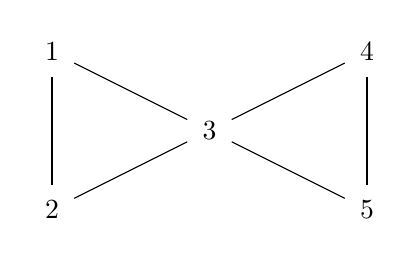
\begin{tikzpicture}
	\node[shape=circle] (1) at (0,0)  {1};
	\node[shape=circle] (2) at (0,-2) {2};
	\node[shape=circle] (3) at (2,-1) {3};
	\node[shape=circle] (4) at (4,0) {4};
	\node[shape=circle] (5) at (4,-2)  {5};
	
	\path [-] (1) edge (2);
	\path [-] (2) edge (3);
	\path [-] (1) edge (3);
	\path [-] (3) edge (4);
	\path [-] (3) edge (5);
	\path [-] (4) edge (5);
\end{tikzpicture}
The left is not a \textit{Eulerian Graph} due to the bridge $\{3,4\}$.\\
The right is a \textit{Eulerian Graph}. A \textit{Eulerian Cycle} can be formed by starting at any node except $3$.\\

\theorem{Degree of Vertices in Eulerian Circuit are Even}
If a graph has an \textit{Eulerian Circuit} then the degree of every vertex in it must be even.\\

\proof{Degree of Vertices in Eulerian Circuit are Even}
If a \textit{Eulerian Circuit} passes through a vertex $v$ $k$ times then $deg_G(v)=2k$.\\

\theorem{Even Degreed Graphs are Composed of Cycles}
Let $G=(V,E)$ be a graph, with $E\neq\emptyset$ \& $\forall\ v\in V\ deg_G(v)$ is even.\\
Then its edge set $E$ can be partitioned into disjoint subsets $E_1,\dots,E_S$, with each $E_i$ being the edge set of a cycle.\\

\proposition{Even Degree $\Leftrightarrow$ Eulerian Graph}
If every vertex of a \textit{Connected Graph} has even degree, then $G$ has a \textit{Eulerian Circuit}.\\
Thus it is a \textit{Eulerian Graph}.\\

\proof{Proposition 4.2}
Let $G=(V,E)$ be a connected graph with $\forall\ v\in V\ deg_G(v)$ being even.\\
If $E=\emptyset$ the result holds trivially.\\
Otherwise, by \textbf{Theorem 4.5}, from some $s\in\nats$ we have disjoint edge sets $E_1,\dots,E_S$ of cycles.\\
For each $i\in[1,s]$ let $V_i$ be the set of vertices contained in the edges $e\in E_i$.\\
If $S=1$ there is nothing to do as the graph is a cycle \& thus \textit{Eulerian}.\\
Otherwise, we use the following process to stitch the cycles together one-by-one to obtain a \textit{Eulerian Circuit}.\\
\\
Define $V_1'=V_1$ \& $E_1'=E_1$.\\
Note that there $\exists\ i\ st\ V_q'\bigcap V_i\neq\emptyset$.\\
Indeed if $V_1\bigcap(V_2\bigcup\dots\bigcup V_S)=\emptyset$ then there would be no edge connecting $V_1'$ to $V_2\bigcup\dots\bigcup V_2$.\\ 
This contradicts the assumption that $G$ is connected.\\
\\
For the least such $i$ choose a vertex $v\in V_1'\bigcap V_i$.\\
Form a circuit by traversing $E_1'$ first, then $E_i$.\\
Let $V_2'=V_1'\bigcup V_i$ \& $E_2'=E_1'\bigcup E_i$, which by contradiction is the edge set of a circuit in which no edge is repeated.\\
\\
Repeat the previous procedure $S-2$ more times to obtain an \textit{Eulerian Circuit} of $G=(V_S',E_S')$.\\

\subsection{Hamiltonian Cycles}

\definition{Hamiltonian Cycle}
Let $G$ be a graph of order $n$.\\
A \textit{Hamiltonian Cycle} in $G$ is a cycle of length $n$.\\
\nb This is a path that visits every edge \& every vertex precisely once.\\

\definition{Hamiltonian Graph}
A graph $G$ is called \textit{Hamiltonian} if it contains a \textit{Hamiltonian Cycle}.\\

\definition{Hamiltonian Path}
A \textit{Hamiltonian Path} in $G$ is a simple path of length $n-1$.\\
\nb This is a path that visits every vertex.\\

\remark{Difficultly of Determining Hamiltonian Graphs}
Deciding whether a graph is \textit{Hamiltonian} or not is $NP$-Complete.\\

\example{Non-Hamiltonian graph with lots of edges}
Let $G$ be $K_{n-1}$ and consider adding one vertex $x_n$ \& one edge $\{x_{n-1},x_n\}$.\\
$G$ is not \textit{Hamiltonian}.\\
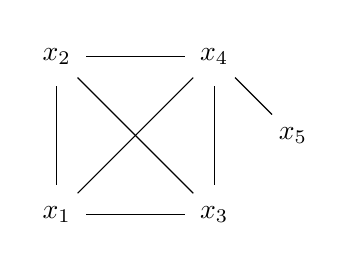
\begin{tikzpicture}
	\node[shape=circle] (1) at (0,0) {$x_1$};
	\node[shape=circle] (2) at (0,2) {$x_2$};
	\node[shape=circle] (3) at (2,0) {$x_3$};
	\node[shape=circle] (4) at (2,2) {$x_4$};
	\node[shape=circle] (5) at (3,1) {$x_5$};
	
	\path [-]
	(1) edge (2)
	(1) edge (3)
	(1) edge (4)
	(2) edge (3)
	(2) edge (4)
	(3) edge (4)
	(4) edge (5);
\end{tikzpicture}

\theorem{Dirac's Theorem}
Let $G$ be a graph of order $n\geq 3$.
\begin{center}
If $\delta(G)\geq\frac{n}{2}$ then $G$ is Hamiltonian.
\end{center}

\proof{Dirac's Theorem}
TODO

\section{Bipartite Graphs}


\definition{Bipartite Graph}
A \textit{Bipartite Graph} is a graph $G=(V,E)$ where the vertex set can be partitioned into two sets $V_1$ \& $V_2$ st $\forall\ \{u,v\}\in E$ we have $u\in V_1$ \& $v\in V_2$.
$$E\subset\{\{u,v\}:u\in V_1,\ v\in V_2\}$$ 

\example{Bipartite Graph}
A path of any length is a \textit{Bipartite Graph}. Below $V_1=\{1,3,5\}$ \& $V_2=\{2,4\}$.\\
\begin{tikzpicture}
	\node[shape=circle] (1) at (0,0) {1};
	\node[shape=circle] (2) at (1,2) {2};
	\node[shape=circle] (3) at (2,0) {3};
	\node[shape=circle] (4) at (3,2) {4};
	\node[shape=circle] (5) at (4,0) {5};
	
	\path [-]
	(1) edge (2)
	(2) edge (3)
	(3) edge (4)
	(4) edge (5);
\end{tikzpicture}

\definition{Complete Bipartite Graph}
A \textit{Complete Bipartite Graph} is a bipartite graph $G=(V_1\bigcup V_2,E)$ where $$\forall\ u\in V_1,\ v\in V_2\ \exists \{u,v\}\in E$$
\textit{i.e} There exists an edge between every element of $V_1$ \& every element of $V_2$ but none within the group.\\
\nb $E=\{\{u,v\}:u\in V_1,v\in V_2\}$.\\

\example{Complete Bipartite Graph}
We have $K_{2,3}$ is\\
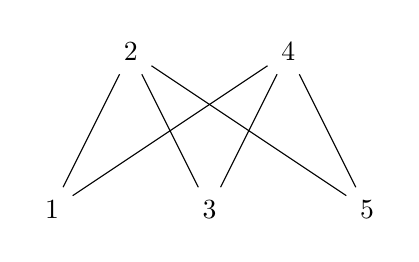
\begin{tikzpicture}
	\node[shape=circle] (1) at (0,0) {1};
	\node[shape=circle] (2) at (1,2) {2};
	\node[shape=circle] (3) at (2,0) {3};
	\node[shape=circle] (4) at (3,2) {4};
	\node[shape=circle] (5) at (4,0) {5};
	
	\path [-]
	(1) edge (2)
	(1) edge (4)
	(3) edge (2)
	(3) edge (4)
	(5) edge (2)
	(5) edge (4);
\end{tikzpicture}

\remark{Even Cycles are Bipartite}
All even cycles are bipartite graphs, since we can partition in the vertices into even \& odd sets.\\

\theorem{Characterisation of Bipartite Graphs}
A graph is bipartite iff it contains no odd cycles.\\

\proof{Characterisation of Bipartite Graphs}
First we shall prove that \textit{A graph is bipartite} $\implies$ \textit{it contains no odd cycles}.\\
It is clear that a bipartite graph contains no odd cycles since a cycle has to alternate between classes/partitions.\\
\begin{tikzpicture}
	\node (1) at (0,0) {$x_{n-1}\in V_1$};
	\node (2) at (0,2) {$x_{n}\in V_2$};
	\node (3) at (2,3) {$x_{n+1}\in ?$};
	\node (4) at (4,2) {$x_{1}\in V_1$};
	\node (5) at (4,0) {$x_{2}\in V_2$};
	
	\path [-]
	(1) edge (2)
	(3) edge (2)
	(3) edge (4)
	(5) edge (4);
\end{tikzpicture}
\\
Now we shall prove that \textit{A graph contains no odd cycles} $\implies$ \textit{It is bipartite}.\\
We assume, without loss of generality, that our graph $G$ is connected.\\
Otherwise we apply the proof to each connected component of $G$ and takes a union of the sets found in the appropriate way:
\\
By assumption $G=(V,E)$ is connected \& contains no odd cycles.\\
Choose $x_0\in V$ and let $X=\{x\in V:d(x_0,x)\mathrm{\ is\ even}\}$ \& $Y=\{y\in V:d(x_0,y)\mathrm{\ is\ odd}\}$ where $d(x,y)$ is the length of the shortest path between $x$ \& $y$.\\
We claim that $X$ \& $Y$ partition $V$ in such a way that all edges of $G$ run between $X$ \& $Y$.\\
This makes $G$ bipartite.\\
\\
Suppose there is an edge $\{y,y'\}$ between two elements of $Y$.\\
Supposing that the length of the shortest path from $x_0\to y=2L+1$ \& $x_0\to y'=2L'+1$.\\
\nb They are both odd since $y,y'\in Y$.\\
Then combining these paths with edge $\{y,y'\}$ to form a circuit of length $2(L+L')+4$ (an odd circuit).\\
But an odd circuit must contain an odd cycle.\\
If $x_1,\dots,x_k,x_1$ is an odd circuit \& $x_i=x_j$ for some $i<j$\\
Then one of $x_i,\dots,x_j$ or $x_j,\dots,x_k,\dots,x_i$ is an odd circuit.\\
If this odd circuit is not a cycle then we continue the decomposition inductively until $k=3$ which is a cycle.\\
\\
This argument shows that no two vertices in the $Y$ are connected by an edge.\\
The same argument applies to $X$.\\
So $G$ is bipartite.\\
\\
Since this argument holds in both directions, they are equivalent.\\

\theorem{Handshaking Lemma}
Let $G=(V_1\bigcup V_2,E)$ be bipartite. Then
$$\sum_{u\in V_1}deg_G(u)=\sum_{v\in V_2}deg_G(v)$$

\proof{Handshaking Lemma}
The number of edges in $G$ is equal to the value of both sides of the equations.\\

\subsection{Hall's Marriage Theorem}

\remark{Motivation}
To model match-making \& scheduling problems using bipartite graphs.\\
\textit{i.e.} As bipartite graph may have vertex classes containing students \& tutorial slots that are feasible due to timetabling.\\
The task is to assign a time slot for a student when they are available \& places in the tutorial is an injective assignment from vertices in one class to the other. (students to time slots).\\

\definition{Neighbourhood of a Set of Vertices}
Let $G=(X\bigcup Y,E)$ be a bipartite graph.\\
For the subset $S\subseteq X$ we define the neighbourhood of $S$ in $G$ to be
$$N_G(S):=\bigcup\limits_{x\in S}N_G(x)$$

\example{Neighbourhood of a Set of Vertices}
In the graph below consider the set $S=\{7,8\}$ then $N_G(S)=\{2,3\}\bigcup\{3,4,5\}=\{2,3,4,5\}$\\
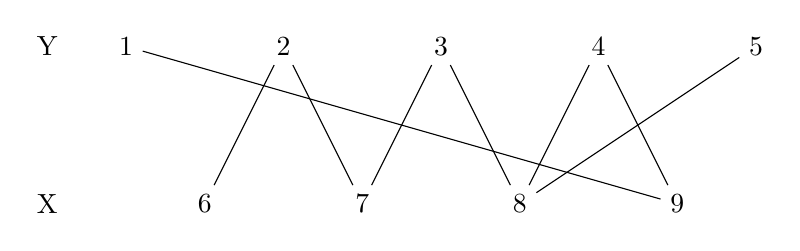
\begin{tikzpicture}
	\node (y) at (0,2) {Y};
	\node (x) at (0,0) {X};
	\node (1) at (1,2) {$1$};
	\node (2) at (3,2) {$2$};
	\node (3) at (5,2) {$3$};
	\node (4) at (7,2) {$4$};
	\node (5) at (9,2) {$5$};
	\node (6) at (2,0) {$6$};
	\node (7) at (4,0) {$7$};
	\node (8) at (6,0) {$8$};
	\node (9) at (8,0) {$9$};
	
	\path [-]
	(1) edge (9)
	(2) edge (6)
	(2) edge (7)
	(3) edge (7)
	(3) edge (8)
	(4) edge (8)
	(4) edge (9)
	(5) edge (8);
\end{tikzpicture}

\definition{Matching}
Let $G=(X\bigcup Y,E)$ be a bipartite graph.\\
A \textit{Matching} from $X$ to $Y$ is a set of edges $\{\{x,y\}:x\in X, y\in Y\}$ which defines an \textit{injective} map with domain $X$ \& co-domain $Y$.\\
\nb There is exactly one edge out of each $x$ \& upto one edge into each $y$.\\

\example{Matching}
Below is a matching from $X$ to $Y$ from the graph in \textbf{Example 5.3}\\
\begin{tikzpicture}
	\node (y) at (0,2) {Y};
	\node (x) at (0,0) {X};
	\node (1) at (1,2) {$1$};
	\node (2) at (3,2) {$2$};
	\node (3) at (5,2) {$3$};
	\node (4) at (7,2) {$4$};
	\node (5) at (9,2) {$5$};
	\node (6) at (2,0) {$6$};
	\node (7) at (4,0) {$7$};
	\node (8) at (6,0) {$8$};
	\node (9) at (8,0) {$9$};
	
	\path [-]
	(1) edge (9)
	(2) edge (6)
	(3) edge (7)
	(4) edge (8);
\end{tikzpicture}

\theorem{Hall's Theorem}
Let $G=(X\bigcup Y,E)$ be a bipartite graph.\\
Then $G$ has a matching from $X$ to $Y$ $\Leftrightarrow\forall\ S\subseteq X,\ |N_G(S)|\geq|S|$.\\

\proof{Theorem 5.3}
First we shall prove that $G$ having a matching from $X$ to $Y\implies\forall\ S\subseteq X,\ |N_G(S)|\geq|S|$.\\
The condition $|N_G(S)|\geq\forall\ S\subseteq X$ is necessary otherwise it would be impossible to match all vertices in $S$ to a vertex in $Y$.\\
\\
Now we shall prove that if $\forall\ S\subseteq X,\ |N_G(S)|\geq|S|\implies\ G$ has a matching.\\
We proceed by induction on the size of $X$.\\
\\
\textit{Base Case}\\
If $|X|=1$ a matching obviously exists as $|N_G(x)|\geq|X|=1$.\\
\\
\textit{Inductive Case}\\
Suppose that $|X|>1$.\\
We distinguish two cases\\
\\
\textit{Case 1}\\
$\forall\ S\subseteq X$ with $S\neq\emptyset$ we have the stronger condition that $|N_G(S)|>|S|$.\\
Choose a vertex $x\in X$ and $y\in Y$ where $\{x,y\}\in E$.\\
Remove $x$, $y$ and any incidence edges to obtain the bipartite graph $G'=(X\backslash\{x\}\bigcup Y\backslash\{y\},E')$.\\
Now the first vertex class $X\backslash\{x\}$ has $|X|-1<|X|$ vertices,\\
Whereas $|N_{G'}(S)|\geq|S|\ \forall\ S\subseteq X\backslash\{x\}$.\\
By our inductive hypothesis $G'$ has a matching and adding the edge $\{x,y\}$ yields the desired matching in $G$.\\
\\
\textit{Case 2}\\
There is a set $S\subseteq X$ with $S\neq\emptyset$ st $|N_G(S)|=|S|$.\\
Consider the bipartite subgraph $G'$ of $G$ which has vertex classes $S$ \& $N_G(S)$ and which contains precisely those edges of $G$ that run between $S$ \& $N_G(S)$.\\
By the inductive hypothesis $G'$ has a matching from $S$ to $N_G(S)$ since $\forall\ T\subseteq S,\ |N_{G'}(T)|=|N_G(T)|\geq|T|$.\\
\\
Now consider $G''$ to be the bipartite subgraph of $G$ which has vertex classes $X\backslash S$ \& $Y\backslash N_G(S)$ and which contains precisley the edges in $G$ that run between these vertex classes.\\

Then we see that $\forall\ T\subseteq X\backslash S$ we have $|N_G(T\bigcup S)\geq|T\bigcup S|=|T|+|S|$ as $S$ \& $T$ are disjoint.\\
But $N_{G''}(T)=N_G(T\bigcup S)\backslash N_G(S)$ so $|N_{G''}(T)|\geq |T|+|S|-|S|=|T|$.\\
Thus, by the inductive hypothesis $G''$ has a matching from $X\backslash S$ to $Y\backslash S$ and by combing this with the matching of $G'$ we obtain a matching for $G$.\\

\remark{Hall's Theorem}
The condition that $|N_G(S)|\geq|S|\ \forall\ S\subseteq X$ is often difficult to verify, except under certain conditions.\\

\theorem{Degree Constrained Hall's Theorem}
Let $G=(X\bigcup Y,E)$ be a bipartite graph.\\
Suppose $\delta(X)>\Delta(Y)$ then $G$ has a matching from $X$ to $Y$.\\

\proof{Degree Constrained Hall's Theorem}
We use double counting.\\
Given any $S\subseteq X$ let $M$ be the number of edges in $G$ between $S$ \& $N_G(S)$ in two different ways
\begin{enumerate}[label=\roman*)]
	\item Counting from the point of view of $S$.
	$$M=\sum_{x\in S}deg_G(x)\geq|S|.\delta(S)$$
	\item Counting from the point of view of $N_G(S)$.
	$$M=\sum_{y\in S}deg_G(y)\leq|S|.\Delta(N_G(S))$$
\end{enumerate}
Thus
$$|N(S)|\geq\frac{M}{\Delta(N_G(S))}\geq\frac{|S|.\delta(S)}{\Delta(N(S))}\geq|S|$$
since $\delta(S)>\Delta(N_G(S))$.\\
Hence the fact there is a matching follows by \textit{Hall's Theorem}.\\

\section{Trees \& Forests}

\definition{Acyclic}
A graph is said to be \textit{Acyclic} if it contains no cycles.\\

\definition{Forest}
A \textit{Forest} is an acyclic graph.\\

\definition{Tree}
A \textit{Tree} is an acyclic connected graph/sub-graph.\\

\example{Forest \& Trees}
Below is an example of a forest on 2 connected components (trees).\\
\begin{tikzpicture}[sibling distance=2em, level distance=2em]
	\node {} 
		child {
			child
			child
			};
\end{tikzpicture}
\begin{tikzpicture}[sibling distance=2em, level distance=2em]
	\node {} 
		child {
			child {
				child
				child
				child
			}
			child
			};
\end{tikzpicture}\\

\remark{Forests are Bipartite}
Any forest (or tree) is bipartite since it contains no odd cycles.\\

\definition{Leaf}
A vertex of degree 1 is called a \textit{Leaf}.\\

\example{Leaf}
In the example below $x_1,x_3\ \&\ x_4$ are leaves.\\
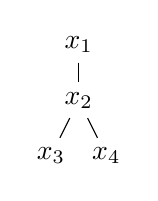
\begin{tikzpicture}[sibling distance=2em, level distance=2em]
	\node {$x_1$} 
		child { node {$x_2$}
			child {node {$x_3$}}
			child {node {$x_4$}}
			};
\end{tikzpicture}\\

\theorem{Guarantee of Leaves}
Every tree on at least 2 vertices has a leaf.\\

\proof{Guarantee of Leaves}
Let $P$ be a maximal simple path in the tree using vertices $x_1,\dots,x_k$.\\
Then $N_G(x_1)\subseteq P$ since the path is maximal.\\
However, $N_G(x)\bigcap P=\{x_2\}$ otherwise we would have a cycle.\\
Hence $N_G(x_1)=\{x_2\}$ and so $x_1$ is a leaf.\\

\remark{Extension of Guarantee of Leaves}
This can be extended to show that such a tree has at least 2 leaves.

\subsection{Basic Properties of Trees \& Forests}

\theorem{Characterisation of Trees}
The following statements are equivalent for a graph $G=(V,E)$
\begin{enumerate}[label=\roman*)]
	\item $G$ is a tree;
	\item $G$ is maximally acyclic (i.e. acyclic \& the addition of any edge creates a cycle);
	\item $G$ is minimally connected (i.e. $G$ is connected \& all edges are bridges);
	\item $G$ is connected \& $|E|=|V|-1$;
	\item $G$ is acyclic \& $|E|=|V|-1$; and,
	\item Any two vertices in $G$ are connected by a unique path.
\end{enumerate}

\proof{Theorem 6.2 - $i)\implies ii)$}
Suppose that $G$ is a tree.\\
Then $G$ is acyclic \& connected.\\
Then $\forall\ x,y\in V\ \exists$ a path from $x$ to $y$.\\
If $\{x,y\}\not\in E$ then the addition of this edge with the previous path becomes a cycle in $G$.\\
Hence $G$ is maximally acyclic.\\

\proof{Theorem 6.2 - $ii)\implies i)$}
Suppose that $G$ is maximally acyclic.\\
Then $G$ is trivially acyclic, thus we want to show that $G$ is connected.\\
Let $x,y\in V$.\\
Then if $\{x,y\}\not\in E$ adding the edge $\{x,y\}$ to $E$ creates a cycle.\\
Thus there must already be a path from $x$ to $y$.\\
Thus $x$ \& $y$ are connected.\\
Since $x$ \& $y$ were chosen arbitrarily then $G$ is connected.\\

\proof{Theorem 6.2 - $i)\implies iii)$}
Suppose that $G$ is a tree.\\
Then $G$ is trivially connected, thus we want to show it is minimally connected.\\
Suppose, to the contrary, that there is an edge $\{x,y\}\in V$, whose removal does not disconnected $G$.\\
Since $H$ with $\{x,y\}$ removed is connected then $G$ contains another path from $x$ to $y$.\\
But this bath with the $\{x,y\}$ would have been a cycle in $G$ contradicting $G$ being acyclic, since it is a tree.\\

\proof{Theorem 6.2 - $i)\implies iv)$}
This is a proof b induction on the size of the vertex set.\\
\textit{Base Case}\\
If $n:=|V|=1$ then there is nothing to prove since there are no edges.\\
\textit{Inductive Case}\\
With $n>1$ we known $G$ contains at least one leaf, $v$.\\
Consider removing $v$ and its incident edge from $G$ to obtain a tree $G'$ on $n-1$ vertices.\\
By the inductive hypothesis $G'$ contains $n-2$ edges.\
Since $v$ has degree $1$ it follow that $G$ has $n-2+1=n-1$ edges.\\
Hence the result holds by mathematical inductions.\\

\proof{Theorem 6.2 - $i)\implies v)$}
Follow from $i)\implies iv)$.\\

\proof{Theorem 6.2 - $i)\implies vi)$}
Suppose that $G$ is a tree.\\
Then $G$ is connected so an two vertices are connected by a path.\\
Suppose that for some $x,y\in V$ there are two distinct paths in $G$ from $x$ to $y$ with
$$P_1:=x=x_1,\dots,x_l=y\\P_2:=x=y_1,\dots,y_m=y$$
Moreover, pick $x$ \& $y$ such that the sum of the lengths of $P_1$ \& $P_2$ is minimal.\\
\textit{Case 1}\\
If $\{x_2,\dots,x_{l-1}\}\bigcap\{y_2,\dots,y_{m-1}\}=\emptyset$ then $P_1$ \& $P_2$ merge to form a cycle.\\
\textit{Case 2}\\
Otherwise, let $i$ be the least index st $x_i\in\{y_2,\dots,y_{m-1}\}$.\\
But as $P_2$ is a path, there is a unique index $j$ st $x_i=y_j$.\\
Hence $x=x_1,x_2,\dots,x_i=y_j,y_{j-1},\dots,y_2,y_1=x$ forms a cycle in $G$ from the two paths.\\
In both cases we have a contradiction as $G$ is a tree \& thus acyclic.\\

\proof{Theorem 6.2 - $vi)\implies i)$}
Suppose that any two vertices are connected by a unique path.\\
Then $G$ is trivially connected, thus we want to show that $G$ is acyclic.\\
It is acyclic since if we have a non-trivial cycle then any two vertices on it would be connected by multiple distinct paths.

\subsection{Spanning Trees \& Applications}

\definition{Spanning Tree}
Let $G=(V,E)$ be a graph.\\
Any tree of the form $T=(V,E')$ with $E'\subseteq E$ is called a spanning tree of $G$.\\

\example{Spanning Tree}
Below is a graph and then a spanning tree of that graph\\
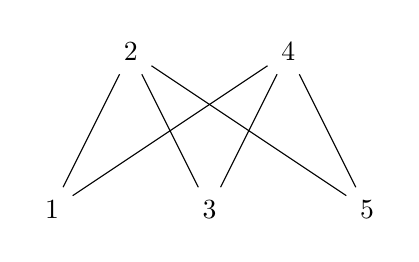
\begin{tikzpicture}
	\node[shape=circle] (1) at (0,0) {1};
	\node[shape=circle] (2) at (1,2) {2};
	\node[shape=circle] (3) at (2,0) {3};
	\node[shape=circle] (4) at (3,2) {4};
	\node[shape=circle] (5) at (4,0) {5};
	
	\path [-]
	(1) edge (2)
	(1) edge (4)
	(3) edge (2)
	(3) edge (4)
	(5) edge (2)
	(5) edge (4);
\end{tikzpicture}
\begin{tikzpicture}
	\node[shape=circle] (1) at (0,0) {1};
	\node[shape=circle] (2) at (1,2) {2};
	\node[shape=circle] (3) at (2,0) {3};
	\node[shape=circle] (4) at (3,2) {4};
	\node[shape=circle] (5) at (4,0) {5};
	
	\path [-]
	(1) edge (2)
	(1) edge (4)
	(3) edge (2)
	(5) edge (4);
\end{tikzpicture}

\theorem{Existence of Spanning Tree}
Every connected graph contains a spanning tree.\\

\definition{Algorithm for Finding Spanning Tree}
Let $G=(V,E)$ be a graph with $n$ vertices and $m$ edges.\\
Order the edges of $G$ arbitrarily into a sequence $e_1,\dots,e_m$.\\
The algorithm constructs sets of edges $E_0,E_1,\dots,\subseteq E$ in stances.\\
Set $E_0=\emptyset$.\\
At state $i$ the algorithm has already defined $E_{i-1}$. Then
$$E_i=\begin{cases}E_{i-1}\bigcup\{e_i\}&\mathrm{If\ graph\ }(V,E_{i-1}\bigcup\{e_i\}\ \mathrm{contains\ no\ cycles}\\E_{i-1}&\mathrm{otherwise}\end{cases}$$
The algorithm stops if after stage $i$ we have that$|E_i|=n-1$.\\
This condition means that $(V,E_i)$ is a tree.\\

\example{Finding Spanning Tree}
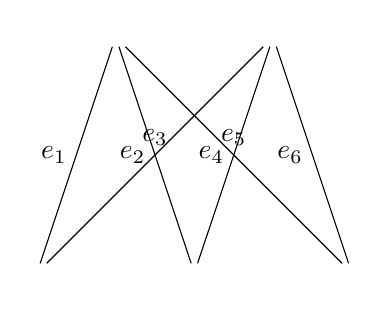
\begin{tikzpicture}
	\node (1) at (0,0) {};
	\node (2) at (1,3) {};
	\node (3) at (2,0) {};
	\node (4) at (3,3) {};
	\node (5) at (4,0) {};
	
	\path [-]
	(1) edge node [left]  {$e_1$} (2)
	(1) edge node [left]  {$e_2$} (4)
	(3) edge node [above] {$e_3$} (2)
	(3) edge node [left]  {$e_4$} (4)
	(5) edge node [above] {$e_5$} (2)
	(5) edge node [left] {$e_6$} (4);
\end{tikzpicture}
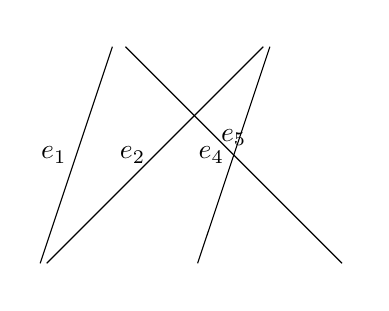
\begin{tikzpicture}
	\node (1) at (0,0) {};
	\node (2) at (1,3) {};
	\node (3) at (2,0) {};
	\node (4) at (3,3) {};
	\node (5) at (4,0) {};
	
	\path [-]
	(1) edge node [left]  {$e_1$} (2)
	(1) edge node [left]  {$e_2$} (4)
	(3) edge node [left]  {$e_4$} (4)
	(5) edge node [above] {$e_5$} (2);
\end{tikzpicture}
\[\begin{array}{ccc}
E_0=\emptyset&E_1=\{e_1\}&E_2=\{e_1,e_2\}\\
E_3=E_2&E_4=\{e_1,e_2,e_4\}&E_5=\{e_1,e_2,e_4,e_5\}
\end{array}\]

\theorem{Correctness of Definition 6.6}
If the algorithm defined in \textbf{Definition 6.6} produces a graph $T$ with $n-1$ edges then $T$ is a spanning tree of $G$.\\
If $T$ has $k<n-1$ edges, then $G$ is a disconnected graph with $n-k$ components.\\

\theorem{Proof of Definition 6.6}
Clearly the algorithm in \textbf{Definition 6.6} produces a graph $T$ with no cycles.\\
We have two cases:\\
\\
\textit{Case 1} - $n-1$ edges.\\
Suppose that $T$ has $n-1$ edges.\\
By $v)\implies i)$ in \textbf{Theorem 6.2}, $T$ is a tree.\\
Since $T$ has the same vertex set as the graph it was produced from, it must be a spanning tree.\\
\\
\textit{Case 2} - $<n-1$ edges.\\
Suppose that $T$ has $k<n-1$ edges.\\
Then $T$ is simply acyclic graph.\\
\textit{i.e} $T$ is a forest whose connected components are trees.\\
We can deduce that $T$ consists of $n-k$ trees.\\
\\
It remains to show that the vertex sets of the connected components of $T$ coincide with the vertex set of the connected components of $G$.\\
Suppose, for the sake of contradiction, $\exists\ x,y\in V$ st $x$ and $y$ lie in the same component of $G$ but in different components of $T$.\\
Say $C_x$ \& $C_y$ respectively.\\
Now consider a path $x=x_1,\dots,x_l=y$ in $G$ from $x$ to $y$.\\
This exists since $x$ \& $y$ are in the same connected component.\\
Let $i$ be the last index for which $x_i$ is contained in $C_x$.\\
Since $y\not\in C_y$ then $i<l$.\\
Thus the edge $e=x_ix_{i+1}$ cannot belong to $T$ since $x_{i+1}\not\in C_x$.\\
This means that $e$ must have formed a cycle with some of the other edges of $T$ already selected at the stage of the algorithm where $e$ is processed.\\
However, the other edges of that cycle form a path from $x_i$ to $x_{i+1}$ in $T$.\\
This contradicts the fact that $x_{i+1}\not\in C_x$.\\
Hence this cannot happen and the connected components of $G$ \& $T$ coincide.\\

\subsection{Minimum Spanning Tree}

\definition{Weight Function}
For a graph $G=(V,E)$ we can define a \textit{Weight Function} $W:E\to\real$.\\

\definition{Weighted Graph}
Let $G=(V,E)$ be a graph \& $W:E\to\real$ be a weight function.\\
If $G$ is equipped with $W$ then $G$ is said to be \textit{Weighted Graph}.\\

\definition{Minimum Spanning Subgraph}
Let $G=(V,E)$ be a connected subgraph equipped with weight function $W:E\to\real$.\\
We say $G'=(V,E')$ with $E'\subseteq E$ is a connected \textit{Minimum Spanning Subgraph} of $G$ when $W(E'):=\sum_{e\in E}W(e)$ is minimised relative to the class of spanning subgraph of $G$.\\

\definition{Minimum Spanning Tree}
A \textit{Minimum Spanning Tree} is a \textit{Minimum Spanning Subgraph} that is also a tree.\\

\remark{Existence of Minimum Spanning Trees}
\begin{itemize}
	\item[-] If the weights of the edges is strictly positive then each \textit{Minimum Spanning Subgraph} must be a \textit{Minimum Spanning Tree}.
	\item[-] If the weights of the edges are non-negative then there is at least one \textit{Minimum Spanning Tree} among the solutions.
\end{itemize}

\definition{Kruskal's Algorithm}
Let $G=(V,E)$ be a connected weighted graph equipped with weight function $W:E\to\real$.\\
Label the edges of $G$ with $e_1,\dots,e_m$, with $m=|E|$, in such a way that
$$W(e_1)\leq\dots\leq W(e_m)$$
Set $E_0=\emptyset$.\\
At state $i$ the algorithm has already defined $E_{i-1}$. Then
$$E_i=\begin{cases}E_{i-1}\bigcup\{e_i\}&\mathrm{If\ graph\ }(V,E_{i-1}\bigcup\{e_i\}\ \mathrm{contains\ no\ cycles}\\E_{i-1}&\mathrm{otherwise}\end{cases}$$
The algorithm stops if after stage $i$ we have that$|E_i|=n-1$.\\
\nb This is the algorithm from \textbf{Definition 6.6}.\\

\proof{Correctness of Kruskal's Algorithm}
Let $G=(V,E)$ and define $n:=|V|$ \& $m:=|E|$.\\
Let $T=(V,E_T)$ be the spanning tree output of \textit{Kruskal's Algorithm}.\\
Let $T=(V,E_T')$ be another spanning tree of $G$.\\
To prove correctness of \textit{Kruskal's Algorithm} we need to show that $W(E_T)\leq W(E_T')$.\\
\\
Suppose that \textit{Kruskal's Algorithm} used the labelling $e_1',\dots,e_m'$ for the edge set $E$, with $w(e_1')\leq\dots\leq w(e_m')$ and outputs the edge set $e_{i_1}',\dots,e_{i_{n-1}}'$.\\
Rename the outputted set as $e_1:=e_{i_1}',\dots,e_{n-1}:=e_{i_{n-1}}'$ for simplicity only.\\
Then we have that
$$W(e_1)\leq\dots\leq w(e_{n-1})\ \&\ E_T=\{e_1,\dots,e_{n-1}\}$$
Let $f_1,\dots,f_{n-1}$ be a labelling on $E_T'$ with $w(t_1)\leq\dots\leq w(t_{n-1})$.\\
It suffices to show that $w(e_i)\leq w(f_i)\ \forall\ i\in\nats^{\leq n-1}$ to prove that $T$ is indeed a minimum spanning tree.\\
\\
Suppose this doesn't hold.\\
Choose the smallest $i$ such that $w(e_i)>w(f_i)$ (\textit{i.e.} Violating the condition).\\
Since the algorithm starts with the edge of least weight \& a single edge cannot form a cycle, thus $i>1$.\\
Consider the edge sets $S:=\{e_1,\dots,e_{i-1}\}$ \& $S':=\{f_1,\dots,f_i\}$.\\
Since $T$ \& $T'$ are trees the graphs $(V,S)$ \& $(V,S')$ are subgraphs of an acyclic graph \& such are acyclic.\\
\\
\textit{Claim}\\
The assumption $w(e_i>w(t_i)\implies\exists\ f\in S'$ st $f$ connects two distinct components of $(V,S)$.\\
The truth of this claim implies that $f\not\in S$ as every edge $e$ in $S$ connects vertices within a single component of $(V,S)$.\\
Moreover, $\left(V,S\bigcup\{f\}\right)$ is still acyclic, whereas $W(f)\leq W(f_i)<W(e_i)$.\\
Thus \textit{Kruskal's Algorithm} would have chosen $f$ instead of $e_i$.\\
This is a contradiction by the definition of the algorithm.\\
\\
\textit{Proof of Claim}\\
Suppose the components of $(V,S)$ have vertex sets $V_1,\dots,V_k$.\\
Then $|D\bigcap\{\{x,y\}:x,y\in V_j\}|=|V_j|-1\ \forall\ j=1,\dots,k$.\\
Summing this equality over all $j$ we get
$$|S|=\sum_{j=1}^k(|V_j|-1)=|V|-k=n-k$$
However, $(V,S')$ is acyclic so $|S'\bigcap\{\{x,y\}:x,y\in V_j\}|\leq |V_j|-1\ \forall\ j=1,\dots,k$\\
since each $(V_j,S'\bigcap\{\{x,y\}:x,y\in V_j\})$ is either a tree or a forest so summing over $j$ we find there are at most $\sum_{j=1}^k(|V_j|-1)=|V|-k=n-k$ elements (edges) of $S'$ connecting vertices within the individual components of $(V,S)$.\\
However
$$|S'|=i=|S|+1=n-k+1$$
hence $\exists\ e\in S'$ that connects distinct components of $(V,S)$.\\
This proves the claim that if $W(e_i)>W(f_i)\implies\exists\ f\in S'$ which connects the components of $(V,S)$.\\
The claim assumes $W(e_i)>W(f_i)$ \& its truth contradicts the definition of \textit{Kruskal's Algorithm}.\\
We conclude that $W(e_i)\leq W(f_i)\ \forall\ i\in\nats^{\leq n-1}$.

\section{Cliques \& Independent Sets}

\theorem{Mantel's Theorem}
Let $G=(V,E)$ be a graph with $n:=|V|$ vertices containing no 3-cycles. Then
\begin{enumerate}[label=\roman*)]
	\item $|E|\leq\left\lfloor\dfrac{n^2}{4}\right\rfloor$;
	\item There exists such a $G$ for which $|E|=\left\lfloor\dfrac{n^2}{4}\right\rfloor$.
\end{enumerate}

\proof{Mantel's Theorem - i)}
This is a proof by induction on the number of vertices $n$.\\
\textit{Base Case}\\
For $n=1$ there are no possible edges
$$\left\lfloor\frac{n^2}{4}\right\rfloor=\left\lfloor\frac{1}{4}\right\rfloor=0=|E|$$
For $n=2$ there is one possible edge
$$\left\lfloor\frac{n^2}{4}\right\rfloor=\left\lfloor\frac{4}{4}\right\rfloor=1\leq|E|$$
The result holds for $n=1,2$.\\
\textit{Inductive Hypothesis}\\
For any graph $G=(V,E)$ with $m:=|E|$ with no 3-cycles we have $|E|\leq\left\lfloor\frac{m^2}{4}\right\rfloor$
\textit{Inductive Case}\\
Let $(G=V,E)$ we a graph with $n:=|E|\geq3$ with no 3-cycles.\\
Let $x,y\in V$ be joined by an edge.\\
Note that if no such pair exists then $|E|=0<\left\lfloor\frac{n^2}{4}\right\rfloor$.\\
\\
\textit{Claim} - $deg_G(x)+deg_G(y)\leq n$.\\
\textit{Proof of Claim}\\
let $A=N_G(x)\backslash\{x,y\}$ and $B=N_G(y)\backslash\{x,y\}$.\\
Consider $deg_G(x)+deg_G(y)\geq n+1$ then
$$|A|+|B|=(deg_G(x)-1)+(deg_G(y)-1)\geq(n+1-2)=n-1$$
But $A\bigcup B\subseteq\{x,y\}$ so
$$n-2=|V\backslash\{x,y\}|\geq|A\bigcup B|=|A|+|B|-|A\bigcap B|\geq(n-1)-|A\bigcap B|$$
Hence $|A\bigcap B|\geq 1$.\\
Pick $z\in A\bigcap B$.\\
Then we have a three cycle $(x,y,z)$ which is a contradiction.\\
Thus the claim is proved.\\
\\
Let $H$ be the graph $G$ with vertices $x,y$ and all incident edges removed.\\
Clearly $H$ contains no $3$-cycles and has $n-2$ vertices, so by our inductive hypothesis $H$ has at most $\left\lfloor\frac{(n-2)^2}{4}\right\rfloor$ edges.\\
Therefore the total number of edges in $G$ is at most
$$\left\lfloor\frac{(n-2)^2}{4}\right\rfloor+deg_G(x)+deg_G(y)-1\leq\left\lfloor\frac{(n-2)^2}{4}\right\rfloor+n-1=\left\lfloor\frac{(n-2)^2+4n-4}{4}\right\rfloor=\left\lfloor\frac{n^2}{4}\right\rfloor$$
Thus by the process of mathematical induction the proof is complete.\\
\nb We subtracted 1 from $deg_G(x)+deg_G(y)$ since otherwise $\{x,y\}$ is counted twice.\\

\proof{Mantel's Theorem - ii)}
It suffices to let $G=K_{\lfloor n/2\rfloor,n-\lfloor n/2\rfloor}=K_{\lfloor n/2\rfloor,\lceil n/2\rceil}$.\\
If $n$ is even then
$$|E|=\frac{n}{2}\times\left(n-\frac{n}{2}\right)=\frac{n^2}{4}=\left\lfloor\frac{n^2}{4}\right\rfloor$$
If $n$ is odd then
$$|E|=\frac{n-1}{2}\left(n-\frac{n-1}{2}\right)=\frac{1}{4}(n62-1)=\frac{n^2}{4}-\frac{1}{4}=\left\lfloor\frac{n^2}{4}\right\rfloor$$

\theorem{}
Let $G=(V,E)$ be a graph with no $3$-cycles.\\
Set $n:=|V|$ \& $|E|=\lfloor n^2/4\rfloor$.\\
Then $G$ is isomorphic to $K_{\lfloor n/2\rfloor,n-\lfloor n/2\rfloor}$

\proof{Theorem 7.2}
This a proof by induction on the number of vertices $n:=|V|$.\\
For $G=(V,E)$ with $|E|=\lfloor n^2/4\rfloor$.\\
\textit{Base Cases}\\
For $n=1$ we have $|E|=\lfloor1/4\rfloor=0$. Then $G\cong K_{0,1}=K_{\lfloor n/2\rfloor,n-\lfloor n/2\rfloor}$.\\
For $n=2$ we have $|E|=\lfloor2^2/4\rfloor=1$. Then $G\cong K_{1,1}=K_{\lfloor n/2\rfloor,n-\lfloor n/2\rfloor}$.\\
\textit{Inductive Case}
Suppose $n\geq3$.\\
Pick an edge $\{x,y\}\in E$ and not that $deg_G(x)+deg_G(y)\leq n$.\\
Let $H$ be the graph which is $G$ with $\{x,y\}$ and all incident edges removed.\\
Note that $H$ can have at most $n-1$ edges fewer than $G$.\\
Hence $|E_H|\geq\lfloor n^2/4\rfloor-(n-1)=\left\lfloor\frac{(n-2)^2}{4}\right\rfloor$.\\
But $H$ has no $3$-cycles on its $n-2$ edges so by \textit{Mantel's Theorem} $|E_H|\leq\left\lfloor\frac{(n-2)^2}{4}\right\rfloor$.\\
Thus $H$ has exactly $\left\lfloor\frac{(n-2)^2}{4}\right\rfloor$ edges.\\
This means that $H$ has exactly $n-1$ edges less than $G$.\\
By the inductive hypothesis $H\cong K_{K_{\lfloor n/2\rfloor,\lceil n/2\rceil}}$.\\
\textit{i.e.} $H$ is a complete bipartite graph on vertex classes $X$ \& $Y$ of size $\lfloor n/2\rfloor$ \& $\lceil n/2\rceil$ respectively.\\
\\
In $G$ $\{x,y\}$ are incident to $n-1$ edges as $deg_G(x)+deg_G(y)=n$.\\
So there are $n-2$ edges connecting $x,y$ to $X\bigcup Y$ since we discount the edge $\{x,y\}$.\\
But $x$ cannot be connected to vertices in both $X$ \& $Y$ otherwise $G$ would contain a $3$-cycle. Hence
$$N_G(x)\backslash\{x,y\}\subseteq X\ \mathrm{or}\ N_G(x)\backslash\{x,y\}\subseteq Y$$
A similar remark applies to $G$, however
$$|X\bigcup Y|=|X|+|Y|=\lfloor n/2\rfloor+\lceil n/2\rceil=\lfloor n/2\rfloor+(n-2)-\lfloor n/2\rfloor=n-2$$
So using $(N_G(x)\backslash\{x,y\})\bigcap(N_G(y)\backslash\{x,y\})=\emptyset$ we have that
$$|H_G(x)\backslash\{x,y\}\bigcup N_G(y)\backslash\{x,y\}|=n-2$$
Thus, we have that $x$ is connected to all vertices in $Y$ and $y$ is connected to all vertices in $X$.\\
\\
Thus $G$ is isomorphic to the complete bipartite graph on vector class $X'$ \& $Y@$ of size $\left\lfloor\frac{n-2}{2}\right\rfloor+1=\left\lfloor\frac{n}{2}\right\rfloor$ and $\left\lceil\frac{n-2}{2}\right\rceil+1=\left\lceil\frac{n}{2}\right\rceil$.

\subsection{Turan's Theorem \& Applications}

\definition{$k$-Partite Graphs}
Let $k\in\nats^{\geq2}$.\\
A graph $G=(V,E)$ is called a \textit{k-Partite Graph} if its vertex set can be partitioned into $k$ pairwise-disjoint vertex classes st $E\subseteq\{\{x,y\}:x\in V_i,y\in V_j; i\neq j\}$.\\

\definition{Complete $k$-Partite Graph}
A graph $G=(V,E)$ is a \textit{Complete k-Partite Graph} if it is $k$-partite \& $E=\{\{x,y\}:x\in V_i,y\in V_j; i\neq j\}$.\\

\example{$k$-Partite Graphs}
Complete $3$-Partite Graph.\\
The graph below has $3$ vertex classes $\{1\},\{2,3\},\{4,5,6\}$.\\
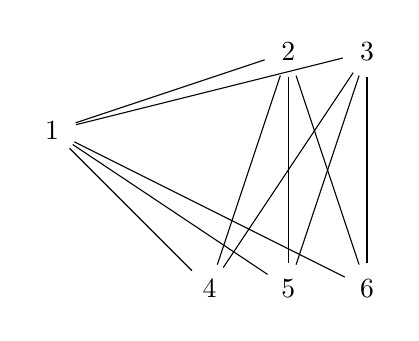
\begin{tikzpicture}
	\node[shape=circle] (1) at (0,0) {1};
	\node[shape=circle] (2) at (3,1) {2};
	\node[shape=circle] (3) at (4,1) {3};
	\node[shape=circle] (4) at (2,-2) {4};
	\node[shape=circle] (5) at (3,-2) {5};
	\node[shape=circle] (6) at (4,-2) {6};
	
	\path [-]
	(1) edge (2)
	    edge (3)
	    edge (4)
	    edge (5)
	    edge (6)
	(2) edge (4)
	    edge (5)
	    edge (6)
	(3) edge (4)
	    edge (5)
	    edge (6);
\end{tikzpicture}

\definition{Turan Graph}
A \textit{Turan Graph} is the graph $T_k(n)$ which is the complete $k$-partite graph on $n$ vertices with vertex classes that are as equal in size as possible.\\
\textit{i.e.} $\left||V_i|-|V_j|\right|\leq1\ \forall\ i,j\in\nats^{\leq k}$.

\example{Turan Graph, $T_3(7)$}
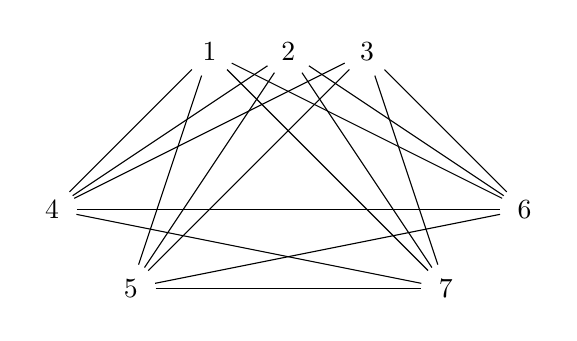
\begin{tikzpicture}
	\node[shape=circle] (1) at (0,0) {1};
	\node[shape=circle] (2) at (1,0) {2};
	\node[shape=circle] (3) at (2,0) {3};
	\node[shape=circle] (4) at (-2,-2) {4};
	\node[shape=circle] (5) at (-1,-3) {5};
	\node[shape=circle] (6) at (4,-2)  {6};
	\node[shape=circle] (7) at (3,-3)  {7};
	
	\path [-]
	(1) edge (4)
		edge (5)
		edge (6)
		edge (7)
	(2) edge (4)
		edge (5)
		edge (6)
		edge (7)
	(3) edge (4)
		edge (5)
		edge (6)
		edge (7)
	(4) edge (6)
		edge (7)
	(5) edge (6)
		edge (7);
\end{tikzpicture}

\remark{Size of Vertex Class in Turan Graph}
In a \textit{Turan Graph} $T_k(n)$ each vertex class has size either $\left\lfloor\frac{n}{k}\right\rfloor$ \& $\left\lceil\frac{n}{k}\right\rceil$.\\

\proof{Remark 7.4}
See handout for lecture 23.\\%TODO

\remark{Degree of Vertices in Turan Graph}
A vertex $x\in V_i$ is joined to every vertex $y\in V\textbackslash V_i$.\\
So $deg_G(x)=|V|-|V_i|$.\\
\nb Vertices of minimum degree are in a vertex class of maximum size \& visa-versa.\\

\proposition{Transforming Turan Graphs}
\begin{itemize}
	\item[-] To obtain $T_k(n-1)$ from $T_k(n)$ remove a vertex from a vertex class of maximum size.
	\item[-] To obtain $T_k(n+1)$ from $T_k(n)$ add a vertex to a vertex class of minimum size.
\end{itemize}

\theorem{}
Let $k\in\nats^{\geq2}$ \& $n\in\nats$.\\
The number of edges of $T_{k}(n)$ is at most
$$\left\lfloor\frac{(k-1)n^2}{2k}\right\rfloor$$

\theorem{Turan's Theorem}
let $G=(V,E)$ be a graph on $n:=|V|$ vertices st $K_k\not\subset G$. Then
$$|E|\leq|E(T_{k-1}(n)|$$

\proof{Turan's Theorem}
We shall prove the following statement for all $k\in\nats^{\geq2}$.
\begin{center}
$S(n):=$"If $G=(V,E)$ is a graph with $n:=|V|$ vertices st $K_k\not\subseteq G$ \& $|E|=|E_{T_{k-1}(n)}|$ then $G$ is isomorphic to $T_{k-1}(n)$."
\end{center}
As $T_{k-1}(n)$ is maximal the statement $S(n)$ implies \textit{Turan's Theorem} on $n$ vertices.\\
\\
We proceed by induction on $n\geq k-1$.\\
let $W_1,\dots,W_{k-1}$ denote the vertex classes of $T_{k-1}(n)$.\\
\textit{Base Case}\\
if $n=k-1$ then each $W_i$ contains precisely one element.\\
Thus $T_{k-1}(n)$ is the complete graph $K_{k-1}$ meaning that $|E|={k-1\choose n}$ so $G\cong K_{k-1}\cong T_{k-1}(n)$.\\
\textit{Inductive Hypothesis} - $S(m)$ holds $\forall\ k-1\leq m<n$.\\
\textit{Inductive Case}\\
Let $x\in V$ st $deg_G(x)=\delta(G)$ and consider $G':=G\backslash x$.\\
Clearly $G'$ is a graph on $n-1$ vertices which does not contain a $K_k$.\\
Using \textbf{Remark 7.2} \& \textbf{Proof 7.6}
$$|E_{g'}|=|E|-\delta(G)\geq|E_{T_{k-1}(n)}|-\delta(T_{k-1}(n)=|E_{T_{k-1}(n-1)}|$$
As $G'$ does not contain a $K_k$ we know, from the inductive hypothesis, that $|E(G')|\leq|E_{T_{k-1}(n-1)}$.\\
Thus $|E(G')|=|E_{T_{k-1}(n-1)}$.\\
By the inductive hypothesis again $G'$ is isomorphic to $T_{k-1}(n-1)$ with vertex classes $V_1,\dots,V_{k-1}$.\\
By proof \textbf{Proof 7.7}.\\
It follow that if $x$ is added to $V_i$ we obtain that $G$ is isomorphic to $T_{k-1}(n)$.\\

\proof{$\delta(G)\leq\delta(T_{k-1}(n)$}
\textit{This is part of the proof of Turan's Theorem}, see proof for definition of $G$.\\
By the handshaking lemma, since $|E|=|E_{T_{k-1}(n)}|$
$$\sum_xdeg_G(x)=\sum_xdeg_{T_{k-1}(n)}(x)\quad(*)$$
Let $m=\delta(T_{k-1}(n))$.\\
Then $\sum_xdeg_{T_{k-1}(n)}(x)=lm+(n-l)(m+1)=n(m+1)-l$ for some $l\in\nats^{\leq n}$.\\
Thus if $\delta(G)<\delta(T_{k-1}(n))$ then $\delta(G)\geq m+1$. So
$$\sum_xdeg_G(x)\geq n\delta(G)\geq n(m+1)>\sum_xdeg_{T_{k-1}}(n)(x)$$
This is a contradiction of $(*)$.\\
Hence $\delta(G)\leq\delta(T_{k-1}(n))$.\\

\proof{For some vertex class $V_i$ of smallest size of $G',\ N_G(x)=\bigcup\limits_{j\neq i}V_j$}
\textit{This is part of the proof of Turan's Theorem}, see proof for definition of $G$.\\
if $x$ is connected to every vertex class $V_j$ in $G'$ we would have a $K_k$ in $G$.\\
Hence $N_G(x)\subseteq\bigcup_{j\neq i}V_j$ for some index $i$.\\
So $|N_G(x)|\leq\left|\bigcup\limits_{j\neq i}V_j\right|$.\\
Since $\delta(G)=\delta(T_{k-1}(n))=n-|W_l|$ where $W_l$ is a vertex class of the greatest cardinality in $T_{k-1}(n)$.\\
It follows $|V_i|=|V_n|$ \& so $|N_G(x)|=\left|\bigcup\limits_{i\neq j}V_i\right|$ using $\left|\bigcup\limits_{i\neq j}V_i\right|=(n-1)-|V_i|$.

\theorem{}
Any graph $G'=(V',E')$ on $n$ vertices with minimum degree $\delta(G')=\left\lfloor\frac{(k-2)n^2}{2(k-1)}\right\rfloor+1$ contains a copy of $K_k$.\\

\theorem{Distances in Bounded Diameters}
Let $x_1,\dots,x_n$ be a finite set of points in the \textit{plane} of diameter $\leq 1$.\\
Then the maximal number of pairs of points whose distance exceeds $\frac{1}{\sqrt{2}}$ is $\lfloor\frac{n^2}{3}\rfloor$.\\

\proof{Theorem 7.6}
Let $G=(V,E)$ be a graph with $V=\{x_1,\dots,x_n\}$ and $E=\{\{x_i,x_j\}:x_i,x_j\in V,|x_i-x_j|>\frac{1}{\sqrt{2}}\}$.\\
We show that $G$ cannot contain a $K_4$ clique since then by \textit{Turan's theorem} $|E|\leq|E_{T_3(n)}|$.\\
But by \textbf{Theorem 7.3} $|E_{T_3(n)}|\leq\left\lfloor\frac{2n^2}{2\times 3}\right\rfloor=\left\lfloor\frac{n^2}{3}\right\rfloor$.\\
So the number of pairs of points whose distinct exceeds $\frac{1}{\sqrt{2}}$ is at most $\left\lfloor\frac{n^2}{3}\right\rfloor$.\\
\\
\textit{Claim} - $G$ does not contain a $K_4$ clique.\\
\textit{Claim of Proof}.\\
Note that any four points in the plane must form one of the following configurations
\begin{enumerate}[label=\roman*)]
	\item A line;\\
	\begin{tikzpicture}
	\node (1) at (0,0) {1};
	\node (2) at (1,0) {2};
	\node (3) at (2,0) {3};
	\node (4) at (3,0) {4};
	
	\path [-]
	(1) edge (2)
	(2)	edge (3)
	(3)	edge (4);
	\end{tikzpicture}
	\item A triangle with an extra point in the middle;\\
	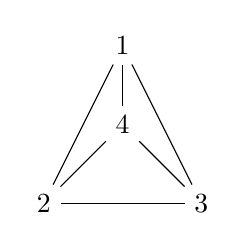
\begin{tikzpicture}
	\node (1) at (0,0)   {1};
	\node (2) at (-1,-2) {2};
	\node (3) at (1,-2)  {3};
	\node (4) at (0,-1)  {4};
	
	\path [-]
	(1) edge (2)
	(1) edge (3)
	(1) edge (4)
	(2)	edge (3)
	(2)	edge (4)
	(3)	edge (4);
	\end{tikzpicture}	
	\item A quadrilateral.\\
	\begin{tikzpicture}
	\node (1) at (0,0)   {1};
	\node (2) at (-1,-2) {2};
	\node (3) at (1,-2)  {3};
	\node (4) at (2,0)  {4};
	
	\path [-]
	(1) edge (2)
	(1) edge (4)
	(2)	edge (3)
	(3)	edge (4);
	\end{tikzpicture}	
\end{enumerate}
In each case three of the points determine an angle of at least $\pi/2$.\\
Consider $x_i,x_j,x_k$ that form this angle.\\
Either $|x_i-x_j|\leq\frac{1}{\sqrt{2}}$ or $|x_j-x_k|\leq\frac{1}{\sqrt{2}}$ otherwise $|x_i-x_k|>1$ which is a contradiction to the assumption of the diameter of the set $x_1,\dots,x_n$.\\
Thus at least one of the edges $\{x_i,x_j\}$ and $\{x_j,x_k\}$ is not present in $G$.\\
This argument holds for any four vertices in $V$.\\
Thus $G$ does not contain a $K_4$ clique.\\
\\
This concludes proof of theorem.\\

\section{Planar Graphs}

\definition{Planar Graphs}
A \textit{Planar Graph} is a graph which can be drawn in a $2D$ plane with no intersecting edges.\\

\definition{Arc}
An \textit{Arc} is a subset of the plane of the form
$$\gamma([0,1])=\{\gamma(x):x\in[0,1])$$
where $\gamma:[0,1]\to\real^2$ is an injective continuous map of the interval $[0,1]$ onto the $2D$ plane.\\
\nb The points $\gamma(0)$ \& $\gamma(1)$ are the \textit{endpoints} of the arc.\\

\example{Arc}
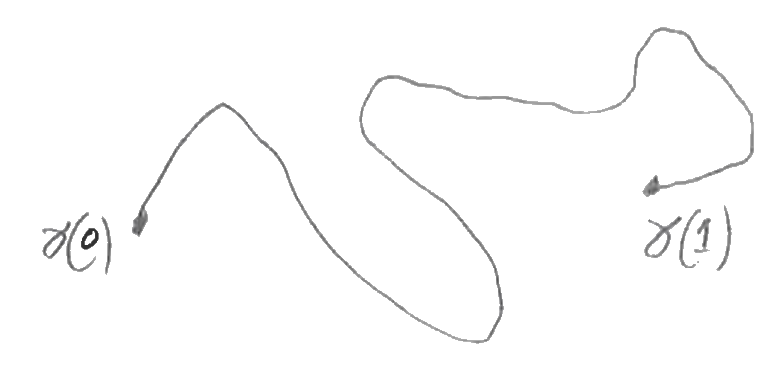
\includegraphics[scale=0.3]{img/arc.png}

\remark{Arcs Don't Intersect Theirselves}
Since $\gamma$ is an injective continuous function then an arc cannot intersect itself.\\

\definition{Drawing of a Graph}
A \textit{Drawing} of a graph $G=(V,E)$ is an assignment of the following form
\begin{enumerate}[label=\roman*)]
	\item For every vertex $V\in V$ assign a point, $p_v$, in the plane in such a way that the map $v\mapsto p_v$ is injective.
	\item For every edge $w=\{x,y\}\in E$ assign an arc $\gamma_e$ in the plane whose endpoints as $p_x$ \& $p_y$ and does not pass through any other points $p_u$ with $u\in V$.\\
\end{enumerate}

\definition{Planar Drawing of Graph}
A \textit{Planar Drawing} of a graph $G=(V,E)$ is a drawing of $G$ where any two arcs, corresponding to distinct edges, do not intersect \& share at most one end point.\\

\example{Planar-Drawing of $K_3$}
Below is a \textit{Planar-Drawing} of $K_3$ on the vertices $\{v_1,v_2,v_3\}$.\\
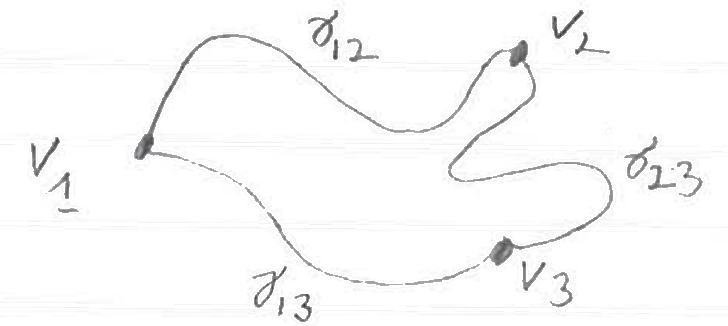
\includegraphics[scale=0.3]{img/planarDrawing.png}

\example{Non-Planar Drawing of $K_3$}
Below is a \textit{Drawing} of $K_3$ on the vertices $\{v_1,v_2,v_3\}$ which is not planar.\\
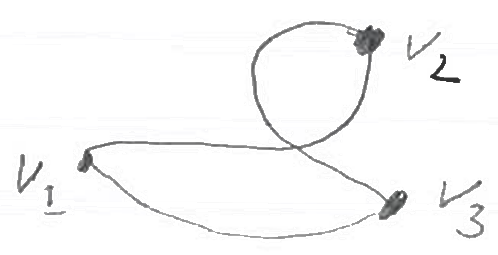
\includegraphics[scale=0.3]{img/nonPlanarDrawing.png}

\definition{Planar Graph}
A \textit{Planar Graph} is a graph that admits at least one \textit{Planar Drawing}.\\

\example{$K_4$ is a Planar Graph}
We usually draw $K_4$ with crossing edges, which is non-planar, but $K_4$ does admit a \textit{Planar Drawing}.\\
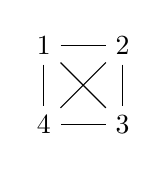
\begin{tikzpicture}
\node (1) at (0,1)   {1};
\node (2) at (1,1) {2};
\node (3) at (1,0)  {3};
\node (4) at (0,0)  {4};
	
\path [-]
(1) edge (2)
(1)	edge (3)
(1) edge (4)
(2)	edge (3)
(2)	edge (4)
(3)	edge (4);
\end{tikzpicture}
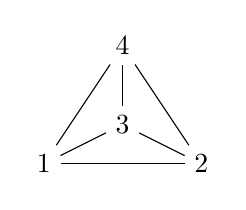
\begin{tikzpicture}
\node (1) at (0,0) {1};
\node (2) at (2,0) {2};
\node (3) at (1,0.5) {3};
\node (4) at (1,1.5) {4};
	
\path [-]
(1) edge (2)
(1)	edge (3)
(1) edge (4)
(2)	edge (3)
(2)	edge (4)
(3)	edge (4);
\end{tikzpicture}

\example{$K_{2,3}$ is a Planar Graph}
We usually draw $K_{2,3}$ with crossing edges, which is non-planar, but $K_4$ does admit a \textit{Planar Drawing}.\\
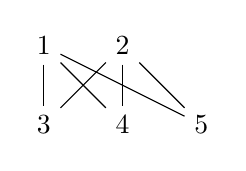
\begin{tikzpicture}
\node (1) at (0,1)   {1};
\node (2) at (1,1)  {2};
\node (3) at (0,0)  {3};
\node (4) at (1,0)  {4};
\node (5) at (2,0)  {5};
	
\path [-]
(1) edge (3)
(1)	edge (4)
(1) edge (5)
(2) edge (3)
(2)	edge (4)
(2) edge (5);
\end{tikzpicture}
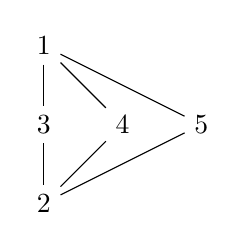
\begin{tikzpicture}
\node (1) at (0,1)   {1};
\node (2) at (0,-1)  {2};
\node (3) at (0,0)  {3};
\node (4) at (1,0)  {4};
\node (5) at (2,0)  {5};
	
\path [-]
(1) edge (3)
(1)	edge (4)
(1) edge (5)
(2) edge (3)
(2)	edge (4)
(2) edge (5);
\end{tikzpicture}

\subsection{Kruatowski's Theoerm}
\textit{We do not cover the full Kruatowski's Theorem in this unit, thus it is non-examinable}.\\

\definition{Jordan Curve}
A \textit{Jordan Curve} is a non-intersecting closed curve in $\real^2$.\\

\theorem{Jordan Curve Theorem}
Any \textit{Jordan Curve} $C$ divides the plane into precisely two connected parts.\\
These parts are called the \textit{Interior} \& \textit{Exterior}.\\
This \textit{Jordan Curve} is called the \textit{Boundary} of both regions.\\

\proof{$K_5$ is not planar}
\textit{This is a proof by contradiction}.\\
Suppose that there is a planar drawing of $K_5$.\\
Let $V_1,\dots,V_5$ be the vertices of $K_5$ and for any $i,j\in\nats^{\leq 5}$ with $i<j$.\\
Let $\gamma_{ij}$ denote the arc connecting $v_i$ \& $v_j$.\\
Since $v_1,v_2,v_4$ form a cycle in $K_5$ the arcs $\gamma_{12},\gamma_{13},\gamma_{23}$ form a \textit{Jordan Curve} $C$.\\
By the \textit{Jordan Curve Theorem} $C$ divides the plane into two regions, interior \& exterior.\\
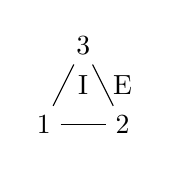
\begin{tikzpicture}
\node (1) at (0,0)   {1};
\node (2) at (1,0)  {2};
\node (3) at (0.5,1)  {3};
\node (E) at (1,0.5)  {E};
\node (I) at (0.5,0.5)  {I};
	
\path [-]
(1) edge (2)
(2)	edge (3)
(3) edge (1);
\end{tikzpicture}\\
Now $v_4$ \& $v_5$ must both lie within the same region, otherwise $\gamma_{45}$ will cross $C$ hence intersecting an arc.\\
Suppose that $v_4$ \& $v_5$ are in the exterior.\\
The arcs $\gamma_{14},\gamma_{24},\gamma_{34}$ partition the exterior of $C$ into 3 regions with the boundary of each region being a \textit{Jordan Curve}.\\
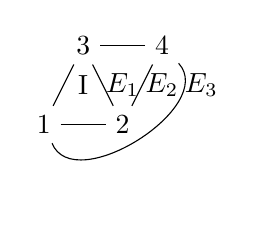
\begin{tikzpicture}
\node (1) at (0,0)   {1};
\node (2) at (1,0)  {2};
\node (3) at (0.5,1)  {3};
\node (4) at (1.5,1)  {4};
\node (E1) at (1,0.5)  {$E_1$};
\node (E2) at (1.5,0.5)  {$E_2$};
\node (E3) at (2,0.5)  {$E_3$};
\node (I) at (0.5,0.5)  {I};
	
\path [-]
(1) edge (2)
(2)	edge (3)
(3) edge (1)
(4) edge[bend left=100] (1)
    edge (2)
    edge (3);
\end{tikzpicture}\\
Suppose, without loss of generality, that $v_5$ lies in $E_1$ with boundary $C$.\\
Now the arc $\gamma_{15}$ has to intersect $C$.\\
This contradicts out assumption that there is a planar drawing of $K_5$ with no intersecting arcs.\\
Thus $K_5$ is not planar.\\

\theorem{Subgraphs of Planar Graphs}
If a subgraph of $G$ is non-planar then $G$ is non-planar.\\

\theorem{Kruatowski's Theorem}
A graph $G$ is planar iff every sub-division of $G$ is planar.\\

\subsection{Euler's Formula}

\definition{Face of a Planar Drawing}
Let $G=(V,E)$ be a planar graph.\\
Consider the set of all points in the plane that lie on none of the arcs of the planar drawing.\\
This set consists of finitely many connected regions, which we call the \textit{Faces of the Drawing}.\\
The region spreading out to infinity is called the \textit{Outer Face} of the drawing \& the remaining faces are called \textit{Inner Faces}.\\

\example{Faces of a Planar Drawing}
Below is a planar drawing of a graph $G$ on 10 vertices which has 5 faces.\\
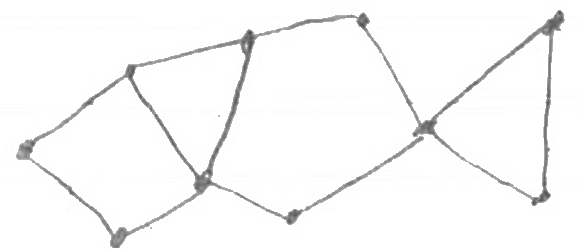
\includegraphics[scale=0.3]{img/faces.png}

\theorem{Euler's Theorem}
let $G=(V,E)$ be a connected graph.\\
Let $F$ be the set of faces of a given planar drawing of $G$. Then
$$|V|-|E|+|F|=2$$
\nb This means the number of faces does not depend on the particular way the drawing is done.\\

\proof{Euler's Theorem}
\textit{This is a proof by induction on the number of edges in $G$}.\\
\textit{Base Case} - $|E|=0$.\\
Note that when $|E|=0$ (i.e. $E=\emptyset$) then, as $G$ is connected it has just one vertex \& so any drawing has just one face.\\
So in the base case $|V|-|E|+|F|=1-0+1=2$.\\
\textit{Inductive Case} - $|E|\geq1$.\\
Here there are $2$ cases to consider
\begin{enumerate}[label=\roman*)]
	\item $G$ contains \underline{no} cycles.\\
	Then $G$ is a tree $\implies|E|=|V|-1$.\\
	Moreover, any planar drawing of a tree has precisely one face.\\
	Thus $|V|-|E|+|F|=|V|-(|V|-1)+1=2$.
	\item $G$ contains at least one cycle.\\
	Fix a cycle and an edge $e\in E$ which belongs to the cycle.\\
	Let $G'=G\backslash e$.\\
	Then $G'$ is connected.\\
	Now consider any planar drawing of $G$ with set of faces $F$,\\
	Removing $e$ yields a planar drawing of $G'$ with faces $F'$.\\
	But, by the inductive hypothesis, in this drawing we have that $|V|-(|E|-1)+|F'|=2$.\\
	However $e$ is adjacent to tow distinct faces of the drawing of $G$, and on removal of $e$ these faces merge into one face of the drawing $G'$.\\
	Therefore $|F'|=|F|-1$. Thus
	$$|V|-|E|+|F|=|V|-|E|+(|F'|+1)=|V|-(|E|-1)+|F'|=2$$
\end{enumerate}
Thus \textit{Euler's Formula} holds forall sizes of $E$.\\

\theorem{Planar Graphs have Few Edges}
Let $G=(V,E)$ be a connected planar graph on at least 4 vertices. Then
$$|E|\leq3|V|-6$$

\proof{Theorem 8.5}
There are two cases
\textit{Case 1} - $|V|=3$.\\
Then there are only $3$ possible edges. Note that $3|V|-6=3\times3-6=9-6=3$ as required.\\
\textit{Case 2} - $|V|\geq 4$.\\
Let $G=(V,E)$ with $|V|\geq4$.\
By the conditions of the theorem $G$ is connected, thus $|E|\geq|V|-1\geq3$.\\
Consider a planar drawing of graph $G$ with set of faces $F$.\\
From \textit{Euler's Formula} we have $|V|-|E|+|F|=2$.\\
We proceed by counting the number, $n$, of pairs $(e,f)$ where $e\in E$ is an edge and $f\in F$ is a face of the drawing and $e$ is adjacent to $f$.\\
\\
Every edge is adjacent to exactly one or two faces.\\
So counting edges first we see that $n\leq2|E|$.\\
Every face is adjacent to at least $4$ edges.\\
This is obvious for bounded faces, but in this case $|E|geq 3$ thus the unbounded face is also clearly adjacent to at least $4$ edges, even when $G$ is a tree.\\
Thus, counting faces first we see that $n\geq3|F|$.\\
It follows that $3|F|\leq N\leq2|E|$.\\
Combining this with \textit{Euler's Formula} we find that
$$|E|=|V|+|F|-2\leq|V|+\frac{2}{3}|E|-2\implies |E|\leq3|V|-6$$

\proof{$K_5$ is not planar}
The graph $K_5$ has $5$ vertices and ${{5}\choose{2}}=10$ edges.\\
By \textbf{Theorem 8.5} if $K_5$ was planar we would have
$$|E|=10\leq3|V|-6=3\times5-6=9$$
Which is clearly untrue.

\section{Graph Colouring}

\subsection{The Chromatic Number of a Graph}

\definition{k-Colouring}
A valid \textit{k-Colouring} of a graph $G=(V,E)$ is an assignment of $k$ colours to each vertex such that no two adjacent vertices have the same colour.\\

\definition{Chromatic Number}
A graph $G$ is said to be \textit{k-Colourable} if it has a \textit{Colouring} that uses at most $k$ colours.\\
The minimum such value of $k$ for graph $G$ is called the \textit{Chromatic Number} of $G$.\\
\nb \textit{Chromatic Number} of $G$ is denoted as $\chi(G)$

\proposition{Common Chromatic Numbers}
Let $m\in\nats$ then $\chi(C_{2m})=2$ \& $\chi(C_{2m-1})=3$.\\
$\forall\ n\in\nats\ \chi(K_n)=n$ since every pair of vertices shares an edge.\\
Let $G$ be a $k$-partite graph then $\chi(G)=k$.\\
Any tree is $2$-partite so all trees are $2$-colourable.\\

\theorem{Chromatic Number \& Max Degree}
For any graph $G=(V,E)$ we have
$$\chi(G)\leq\Delta(G)+1$$
This means that $\forall\ k\in\nats$ with $k\geq\Delta(G)$ we have $\chi(G)\leq k+1\implies G$ is $(k+1)$-colourable.\\

\proof{Theorem 9.1}
We proceed by induction on $n:|V|$.\\
\textit{Base Case} - $n=1$.\\
Suppose that $G=(V,E)$ is such that $|V|=1$.\\
Then $\Delta(G)=0$ \& $G$ is trivially $1=0+1+\Delta(G)+1$ colourable.\\
So $\chi(G)=\Delta(G)+1$ in this case.\\
\textit{Inductive Case} - $n>1$.\\
Suppose that $G=(V,E)$ is a graph with $|V|>1$.\\
The inductive hypothesis states that $\chi(\hat{G})\leq\Delta(\hat{G})+1\ \forall\ \hat{G}=(\hat{V},\hat{E})$ where $|\hat{V}|<|V|$.\\
Choose a vertex $x\in V$ \& remove $x$ and all its adjacent edges from $G$ to form the graph $G'=G\backslash x$ on $n-1$ vertices.\\
Clearly $\Delta(G')\leq\Delta(G)$.\\
By the inductive hypothesis $\chi(G')\leq\Delta(G')+1$.\\
Noting that $\chi(G')\leq\Delta(G')+1\leq\Delta(G)+1$.\\
Thus $G'$ can be coloured with at most $\Delta(G)+1$ colours.\\
Consider the neighbouring vertices of $x$ in $G$, of which there are at most $\Delta(G)$.\\
Thus, if we fix a valid $\Delta(G)+1$ colouring of $G'$ these neighbours use at most $\Delta(G)$ colours, leaving at least $1$ colour for $x$.\\
Thus $G$ is itself $\Delta(G)+1$ colourable.\\
Thus $\chi(G)\leq\Delta(G)+1$.\\

\remark{$\chi(G)$ is not necessarily close to $\Delta(G)+1$}
Consider a star shaped graph on $n$ vertices.\\
Then $\Delta(G)=n-1$ but $\chi(G)=2\ \forall\ n$.\\

\theorem{The Four-Colour Theorem}
At most four colours are required to colour a map in such a way that no two adjacent territories are coloured.\\
\nb We prove a weaker statement.\\

\theorem{The Five-Colour Theorem}
At most five colours are required to colour a map in such a way that no two adjacent territories are coloured.\\

\remark{Assumptions for Five-Colour Theorem}
We make the following assumptions about the region which forms the mapped referred to in the \textit{Five-Colour Theorem}
\begin{enumerate}[label=\roman*)]
	\item Each state is assumed to be connected region. (\textit{i.e.} No state is formed of two regions).
	\item Two states are neighbours only if they share a continuous interval of a border. (\textit{i.e.} Regions do not meet at a point, rather than a line).
\end{enumerate}

\proposition{A Map as a Planar Drawing}
We can view a map as a planar drawing of a graph $G$ in which the faces correspond to the countries and the edges correspond to borders between them.\\
The vertices of $G$ are points lying on the border of $4$ or more states.\\

\proposition{Colouring of the Map verse Colouring of the Dual-Graph of $G$}
Note that a $k$-colouring of a map of countries can be though of as a valid $k$-colouring of the capital cities of these countries where any two capitals of a country with a common border must be different colours.\\

\definition{Informal Definition of Dual-Graph}
Let $G=(V,E)$ is a planar graph, with a planar drawing of $G$.\\
The dual-graph $G^*:=(V^*,E^*)$, relative to the planar drawing, is obtained by drawing one vertex inside each face of $G$ and connecting two vertices $u,v\in V^*$ by the edge $\{u,v\}\in E^*$ if the two corresponding faces share a common edge $e\in E$.\\

\example{Dual-Graph}
Below is a planar drawing of $G=K_{2,3}$ \& its dual-graph $G^*$.\\
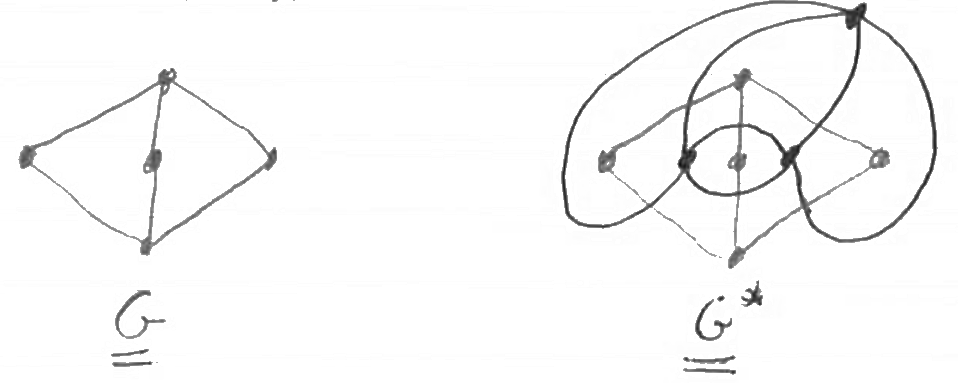
\includegraphics[scale=0.3]{img/dual.png}

\remark{Double Edges in Dual-Graphs}
$G^*$ in \textbf{Example 9.1} has double edges (\textit{i.e.} multiple edges between the same pair of vertices).\\
For the purpose of analysing colourings of the vertices of a dual-graph we can ignore the extra edges.\\

\proposition{Using Dual-Graphs}
Consider a map $G$ \& its dual-graph $G^*$, simplify $G^*$ as described in \textbf{Remark 9.3}.\\
A valid colouring of the faces of $G$ corresponds to a valid colouring of the vertices of $G^*$.\\
Thus there is a $k$-colouring of the $G$ iff there is a $k$-colouring of the $G^*$.\\
\nb Thus proving the \textit{Five-Colour Theorem} is equivalent to showing that every planar graph s $5$-colourable.\\

\proof{The Five-Colour Theorem}
We shall prove this by induction on $n:=|V|$.\\
\textit{Base Case} - $n\in[0,5]$.\\
When $n\leq5$ the result is trivially true.\\
\textit{Inductive Hypothesis}\\
Any planar graph $\hat{G}=(\hat{V},\hat{E})$ with $|\hat{V}|<n$ than $\chi(\hat{G})\leq5$.\\
\textit{Inductive Case} - $n>5$.\\
Suppose $n>5$.\\
By problem 9 on sheet 9, any connected planar graph has a vertex of degree $\leq5$.\\
Thus $G$ most contain a vertex $v\in V$ with $deg_Gv\leq5$.\\
Note that if $G$ is not connected, there is one such vertex in every component of $G$.\\
We can distinguish 2 cases\\
\\
\textit{Case 1}\\
Consider when $deg_G(v)<5$.\\
Let $G'=G\backslash v$.\\
The graph $G'$ is a planar graph on $n-1$ vertices \& by the inductive hypothesis can be coloured with at most 5 colours.\\
Since $v$ has $<5$ neighbours there is at least one unused colours among its neighbours, this colour can be assigned to $v$.\\
Thus $G$, in this case, is $5$-colourable (\textit{i.e} - $\chi(G)\leq5$).\\
\\
\textit{Case 2}\\
Consider when $deg_G(v)=5$.\\
Fix a planar drawing of $G$ \& let $t,u,x,y,z$ be the neighbours of $v$ in clockwise order.\\
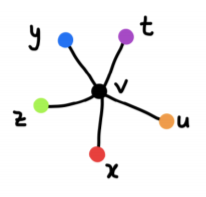
\includegraphics[scale=0.5]{img/5proof1.png}\\
By the inductive hypothesis $G':=G\backslash v$ can be coloured by at most $5$ colours.\\
Suppose that this colouring is given by assignment $C:V\backslash\{v\}\to\{1,2,3,4,5\}$.\\
If the neighbours of $v$ in $G'$ only use colours then result is proved as in \textit{Case 1}.\\
Thus, we must consider when $v$'s neighbours has a unique colour, so all $5$ are used.\\
Let $C_{x,y}=\{v\in V':c(c)=c(x)\ or\ c(c)=c(y)\}$ \textit{i.e} $C_{x,y}$ is the set of vertices in $G'$ that are coloured red or blue in examples.\\
We have two sub-cases\\
\\
\textit{Case 2a)}\\
Consider when there is no path from $x$ to $y$ in $G'$ using only vertices in $C_{x,y}$.\\
Let $C_{x,y}'$ be the set of all vertices $w\in V'$ that can be reached via a path from $x$, using only vertices in $C_{x,y}$.\\
By our assumption, $Y\not\in C_{x,y}'$.\\
However, this means that we can define a new colouring $c'$ of $G'$ by simply switching the colours of vertices in $C'_{x,y}$ as below\\
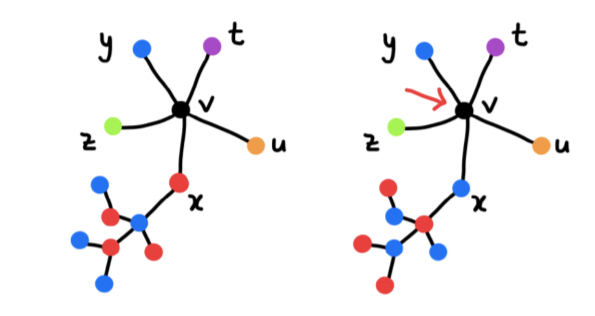
\includegraphics[scale=0.5]{img/5proof2.png}\\
Meaning $x$ \& $y$ have the same colour, since only $x$ is flipped, thus the neighbours of $v$ use $5-1=4$ colours.\\
The result is proved similarly to \textit{Case 1}.\\
\\
\textit{Case 2b}
Consider when there is a path $P$ $x$ to $y$ in $G'$ using only vertices in $C_{x,y}$.\\
Let $C_{z,t}:=\{v\in V':c(v)=c(z)\ or\ c(v)=c(t)\}$ \textit{i.e.} the set of all vertices that are green or purple.\\
Clearly $C_{x,y}\cap C_{z,t}=\neg$.\\
The edges $\{v,x\}$ \& $\{v,y\}$ together with the path $P$ form a cycle in $G$ which gives rise to a \textit{Jordan Curve} in the drawing of $G$.\\
Without loss of generality the vertex $z$ lies in the interior of this curve \& vertex $t$ lies in its exterior.\\
Thus, any path from $z$ to $t$ in $G'$ must use a vertex, from the cycle, coloured red or blue.\\
Thus, it follows that there is no path from $z$ to $t$ in $G'$ using only vertices from $C_{z,t}$.\\
However, this is exactly the same as \textit{Case 2a} with $z$ \& $t$ replacing $x$ \& $y$ and the swapping the colours.\\
Thus, $z$ \& $t$ can be the same colour meaning the neighbours of $v$ use only $5-1=4$ colours, leaving a colour for $v$.\\
\\
This shows that the \textit{Five-Colour Theorem} holds in all cases.

\section{Order from Disorder}

\subsection{Ramsey's Theorem}

\definition{Ramsey Number}
The \textit{Ramsey Number} for $s\in\nats^{\geq2}$, $r(s)$, is the least $n\in\nats$ st $\forall$ $2$-colourings of the \underline{edges} of $K_n\ \exists$ a \textit{Monochromatic} $K_s$ subgraph.\\

\theorem{$r(3)=6$}

\definition{Off-Diagonal Ramsey Number}
The \textit{Off-Diagonal Ramsey Number} for $s,t\in\nats$, $r(s,t)$ is the least $n\in\nats$ st $\forall$ $2$-Colourings of the \underline{edges} of $K_n\ \exists$ a \textit{Monochromatic} $K_s$ \textbf{or} $K_t$ subgraph .\\

\theorem{Off-Diagonal Ramsey Number Identities}
\[\begin{array}{rcll}
r(s,s)&=&r(s)&\forall\ s\in\nats\\
r(s,t)&=&r(t,s)&\forall\ s,t\in\nats\\
r(2,t)&=&t&\forall\ t\in\nats
\end{array}\]

\theorem{Ramsey's Theorem}
The \textit{Off-Diagonal Ramsey Number} $r(s,t)$ exists $\forall\ s,t\in\nats^{\geq2}$. Moreover,
$$r(s,t)\leq r(s-1,t)+r(s,t-1)\ \forall\ s,t\in\nats^{\geq3}$$

\proof{Ramsey's Theorem}
Since $r(2,t)=t)\ \&\ r(s,2)=s$ it suffices to show that, for $s,t\in\nats^{\geq3}$, if $r(s-1,t)\ \&\ r(s,t-1)$ exist then $r(s,t)\leq r(s-1,t)+r(s,t-1)$ since then, by induction on $s+t$ we have $r(s,t)$ exists $\forall\ s,t\in\nats^{\geq2}$.\\
\\
Define $a:=r(s-1,t)$ \& $b:=r(s,t-1)$.\\
Consider an arbitrary red/blue colouring $C$ of $K_{a+b}$.\\
We must show that it contains a red $K_s$ or a blue $K_t$.\\
Fix some vertex $x\in V_{K_{a+b}}$.\\
Since $x$ has $a+b-1$ neighbours there must be either at least $a$ red edges \textbf{or} $b$ blue edges incident with $x$.\\
Suppose the former is true.\\
In the latter case we are done.\\
In the former case, we obtain a red $K_s$ by adjoining $x$ to this red $K_{s-1}$.\\
Now we are done in both cases.\\

\theorem{Upper Bound on Ramsey Number}
$\forall\ s\in\nats^{\geq2},\ r(s)$ exists. Further
$$r(s)\leq r(s-1,s)+r(s,s-1)=2r(s-1,s)\ \forall\ s\in\nats^{\geq3}$$ 

\subsection{Bounds on Ramsey Numbers}

\remark{Few Ramsey Numbers are known}
The only know \textit{Ramsey Numbers} are $r(3);\ r(3,4);\ r(3,5);\ r(3,6);\ r(3,7);\ r(3,8);\ r(3,9); r(4);\ \&,\ r(4,5)$.\\

\theorem{Upper Bound on Ramsey Number}
\textit{This is non-examinable}.\\
If $r(s-1,t)\ \&\ r(s,t-1)$ are both even then
$$r(s,t)<r(s-1,t)+r(s,t-1)$$
\nb - This is a strict inequality.\\

\proof{$r(4)=18$}
\textit{In Problem Sheet 10, Q7 it is proved that $r(4)>17$}.\\
Notice that $r(2,4)=4\ \&\ r(3,3)=6$.
\[\begin{array}{rrcl}
\implies&r(3,4)&<&r(2,4)+r(3,3)\\
&&=&4+6\\
&&=&10\\
\implies&r(3,4)&\leq&9\\
\implies&r(4)&\leq&r(3,4)+r(4,3)\\
&&=&2r(3,4)\\
&&\leq&18\\
\implies&r(4)&\leq&18
\end{array}\]
Since $17<r(4)\leq 18\implies r(4)=18$.\\

\proposition{Upper bound on Ramsey Numbers}
$\forall\ s,t\geq2$ we have $r(s,t)\leq2^{s+t}$.\\
Equivalently, $r(s)<4^s$.\\

\proof{Proposition 10.1}
\textit{This is a proof by induction on $s+t$}.\\
\textit{Base Case} - $s=t=2$\\
By \textbf{Theorem 10.2} if $s=2$ then $r(s,t)=t<2^{s+t}$, likewise if $t=2$ then $r(s,t)<2^{s+t}$.\\
So $r(s,t)\leq2^{s+t}$ for $s=t=2$.\\
\textit{Inductive Assumption} - $\forall\ s,t>2\ \&\ s',t'\geq2$ with $s'+t'<s+t$ then $r(s',t')<2^{s'+t'}$.\\
\textit{Inductive Step}\\
By \textbf{Theorem 10.3} $r(s,t)\leq r(s-1,t)+r(s,t-1)$.\\
We apply the inductive hypothesis to both terms on the right of this inequality.
\[\begin{array}{rcl}
r(s,t)&\leq&2^{s-1+t}+2^{s+t-1}\\
&=&2\times2^{s+t-1}\\
&=&2^{s+t}
\end{array}\]

\remark{Lower Bounds on Ramsey Numbers are non-examinable}

\newpage
\setcounter{section}{-1}
\section{Reference}

\subsection{Notation}

\notation{Adjacent Vertices}
If $\{u,v\}\in G$ then we write $$u\sim v$$

\notation{Binomial Coefficient}
Let $n,k\in\nats_0$. We denoted the \textit{Binomial Coefficient} of $n$ wrt $k$ by
$$\begin{pmatrix}n\\k\end{pmatrix}$$
This is pronounced \textit{`n choose k'}.\\

\notation{Bipartite Graph}
A bipartite graph with vertex sets $V_1$ \& $V_2$ is denoted by
$$G=(V_1\bigcup V_2,E)$$

\notation{Complete Bipartite Graph}
A complete bipartite graph with vertex sets $V_1$ \& $V_2$ where $|V_1|=n$ \& $|V_2|=m$ is denoted by
$$K_{m,n}$$

\notation{Complete Graph}
A complete graph of order $n$ is denoted by
$$K_n$$

\notation{Cycle}
A cycle of length $n$ is denoted by $$C_n$$

\notation{Degree}
Let $G=(V,E)$ be a graph \& $v\in V$. We denote the \textit{Degree} of $v$ by
$$deg_G(v)$$

\notation{Disjoint Union Notation}
The following notation denotes the union of disjoint sets
$$\bigsqcup$$

\notation{Generating Function}
We denote that $f(x)$ is the generating function of the sequence $(a_0,a_1,a_2,\dots)$ by
$$(a_0,a_1,a_2,\dots)\rightleftarrows f(x)$$

\notation{Maximum Degree}
For a graph $G=(V,E)$ we define its maximum degree as
$$\Delta(G):=\mathrm{max}\{deg_G(v):v\in V\}$$

\notation{Minimum Degree}
For a graph $G=(V,E)$ we define its minimum degree as
$$\delta(G):=\mathrm{min}\{deg_G(v):v\in V\}$$

\notation{Neighbourhood}
Let $G=(V,E)$ be a graph \& $v\in V$. We denote the \textit{Neighbourhood} of $v$ by
$$N_G(v)$$

\notation{Path}
A path of length $n$ is denoted by $$P_n$$

\notation{Reduced Factorial}%RENAME THIS
$$(n)_k:=n\times(n-1)\times\dots\times(n-k+1)=\dfrac{n!}{(n-k)!}$$
\nb $(n)_n=n!$.\\

\notation{Set of Initial Natural Numbers}
Let $n\in\nats$. Then
$$[n]:=[x|x\in\nats, 1\leq x\leq n]$$
\end{document}
